%%% Hlavní soubor. Zde se definují základní parametry a odkazuje se na ostatní části. %%%

%% Verze pro jednostranný tisk:
% Okraje: levý 40mm, pravý 25mm, horní a dolní 25mm
% (ale pozor, LaTeX si sám přidává 1in)
\documentclass[a4paper,oneside,12pt]{report}
\setlength\textwidth{155mm}
\setlength\textheight{247mm}
%\setlength\oddsidemargin{00mm}
\setlength\topmargin{-10mm}
\setlength\headheight{0mm}
\setlength\oddsidemargin{05mm}
\setlength\evensidemargin{05mm}
\let\openright=\clearpage


%% Vytváříme PDF/A-2u
\usepackage[a-2u]{pdfx}

%% Přepneme na českou sazbu a fonty Latin Modern
\usepackage[czech]{babel}
\usepackage{lmodern}
\usepackage[T1]{fontenc}
\usepackage{textcomp}

%% Použité kódování znaků: obvykle latin2, cp1250 nebo utf8:
\usepackage[utf8]{inputenc}

%%% Další užitečné balíčky (jsou součástí běžnýsrov.stribucí LaTeXu)
\usepackage{amsmath}        % rozšíření pro sazbu matematiky
\usepackage{amsfonts}       % matematické fonty
\usepackage{amsthm}         % sazba vět, definic apod.
\usepackage{bbding}         % balíček s nejrůznějšími symboly
			   										% (čtverečky, hvězdičky, tužtičky, nůžtičky, ...)
\usepackage{bm}             % tučné symboly (příkaz \bm)
\usepackage{graphicx}       % vkládání obrázků
\usepackage{fancyhdr}				% možnost slylizovat záhlaví
\usepackage{fancyvrb}       % vylepšené prostředí pro strojové písmo
\usepackage{indentfirst}    % zavede odsazení 1. odstavce kapitoly
\usepackage[nottoc]{tocbibind} % zajistí přidání seznamu literatury,
\usepackage{icomma}         % inteligetní čárka v matematickém módu
\usepackage{dcolumn}        % lepší zarovnání sloupců v tabulkách
\usepackage{booktabs}       % lepší vodorovné linky v tabulkách
\usepackage{paralist}       % lepší enumerate a itemize
\usepackage{caption}				%	popisky
\usepackage{dirtree}				% strom souborů
\usepackage[bottom]{footmisc}  % poznámky pod čarou vespod
\usepackage{bibentry}
\usepackage{xurl}						% umožní url zalomit všude
\nobibliography*

\usepackage{color}
\usepackage{forest}					% na rodokmeny
\usepackage{natbib}
%\setbibentrystyle{author}

\definecolor{pblue}{rgb}{0.13,0.13,1}
\definecolor{pgreen}{rgb}{0,0.5,0}
\definecolor{pred}{rgb}{0.9,0,0}
\definecolor{pgrey}{rgb}{0.46,0.45,0.48}
\renewcommand{\baselinestretch}{1.5}
%%% Údaje o práci

\def\NazevSkoly{Gymnázium, Praha 6, Arabská 14}
% Název oboru včetně počátečního 'Obor'.
\def\NazevOboru{Dějepis}

% Název práce v jazyce práce (přesně podle zadání)
\def\NazevPrace{Židovké město v Třebíči}

% Název práce v angličtině
\def\NazevPraceEN{Jewish town in Třebíč}

% Název práce v němčině
\def\NazevPraceDE{Jüdische Stadt in Třebíč}

% Jméno auto
\def\AutorPrace{Havránek Kryštof 2.E}

% Rok odevzdání
\def\RokOdevzdani{2020}
% Měsíc odevzdání
\def\MesicOdevzdani{Březen}

% Vedoucí práce: Jméno a příjmení s~tituly
\def\Vedouci{PhDr. Lenka Dvořáková }

% Nepovinné poděkování (vedoucímu práce, konzultantovi, tomu, kdo
% zapůjčil software, literaturu apod.)
\def\Podekovani{%
\textbf{Poděkování}

Děkuji Paní profesorce PhDr. Lence Dvořákovákové za pomoc při psaní práce.
Děkuji také židovskému muzeu ve Třebíči, za poskytnutí bakalářských prací a dalších zdrojů, jenž jsem sám nenašel.
}

% Abstrakt (doporučený rozsah cca 80-200 slov; nejedná se o zadání práce)
\def\Abstrakt{%
Práce pojednává o Židovském městě ve Třebíči.
Jako první prochází historii celého města Třebíč poté se zaměřuje pouze na město židovské.
U něho probírá dějiny od raných počátků židovského osídlení přes tvorbu ghetta po konec osídlení způsobený nacistickou genocidou.
Zmapuje také vztahy mezi šlechtou, měšťanstvem a Židy a jak se vyvíjeli v průběhu historie.
Nakonec popíše dějiny několika staveb v Židovském městě.
}
\def\AbstraktEN{%
Main topic of this paper is the Jewish town in Třebíč.
At the beginning it goes trough history of Třebíč as a whole and later focuses solely on Jewish town.
In chapters dedicated to Jewish town paper first describes towns history form the beginning of Jewish settlement here to end of Jewish community caused by the Nazi genocide.
After that it takes closer look on relations between aristocracy, Jewry and town folk and how they changed in coure of history.
In the end paper describes history of few buildings in Jewish town.
}
\def\AbstraktDE{%
}

% 3 až 5 klíčových slov (doporučeno), každé uzavřeno ve složených závorkách
\def\KlicovaSlova{%
	{Třebíč}, {Židovstvo}, {Židé na Moravě}, {Historie Židovstva}, {Podklášteří}
}
\def\KlicovaSlovaEN{%
	{Trebitsh}, {Jewry}, {Jews in Moravia}, {Jewsish history}, {Podklášteří}
}

\def\KlicovaSlovaDE{%
}

%% Balíček hyperref, kterým jdou vyrábět klikací odkazy v PDF,
%% ale hlavně ho používáme k uložení metadat do PDF (včetně obsahu).
%% Většinu nastavítek přednastaví balíček pdfx.
\hypersetup{unicode}
\hypersetup{breaklinks=true}

%% Definice různých užitečných maker (viz popis uvnitř souboru)
%%% Tento soubor obsahuje definice různých užitečných maker a prostředí %%%
%%% Další makra připisujte sem, ať nepřekáží v ostatních souborech.     %%%

%%% Drobné úpravy stylu

% Tato makra přesvědčují mírně ošklivým trikem LaTeX, aby hlavičky kapitol
% sázel příčetněji a nevynechával nad nimi spoustu místa. Směle ignorujte.
\makeatletter
\def\@makechapterhead#1{
  {\parindent \z@ \raggedright \normalfont
   \Huge\bfseries \thechapter. #1
   \par\nobreak
   \vskip 20\p@
}}
\def\@makeschapterhead#1{
  {\parindent \z@ \raggedright \normalfont
   \Huge\bfseries #1
   \par\nobreak
   \vskip 20\p@
}}
\makeatother

% Toto makro definuje kapitolu, která není očíslovaná, ale je uvedena v obsahu.
\def\chapwithtoc#1{
\chapter*{#1}
\addcontentsline{toc}{chapter}{#1}
}

% Trochu volnější nastavení dělení slov, než je default.
\lefthyphenmin=2
\righthyphenmin=2

% Zapne černé "slimáky" na koncích řádků, které přetekly, abychom si
% jich lépe všimli.
\overfullrule=1mm

%%% Makra pro definice, věty, tvrzení, příklady, ... (vyžaduje baliček amsthm)

\theoremstyle{plain}
\newtheorem{veta}{Věta}
\newtheorem{lemma}[veta]{Lemma}
\newtheorem{tvrz}[veta]{Tvrzení}

\theoremstyle{plain}
\newtheorem{definice}{Definice}

\theoremstyle{remark}
\newtheorem*{dusl}{Důsledek}
\newtheorem*{pozn}{Poznámka}
\newtheorem*{prikl}{Příklad}

%%% Prostředí pro důkazy

\newenvironment{dukaz}{
  \par\medskip\noindent
  \textit{Důkaz}.
}{
\newline
\rightline{$\square$}  % nebo \SquareCastShadowBottomRight z balíčku bbding
}

%%% Prostředí pro sazbu kódu, případně vstupu/výstupu počítačových
%%% programů. (Vyžaduje balíček fancyvrb -- fancy verbatim.)

\DefineVerbatimEnvironment{code}{Verbatim}{fontsize=\small, frame=single}

%%% Prostor reálných, resp. přirozených čísel
\newcommand{\R}{\mathbb{R}}
\newcommand{\N}{\mathbb{N}}

%%% Užitečné operátory pro statistiku a pravděpodobnost
\DeclareMathOperator{\pr}{\textsf{P}}
\DeclareMathOperator{\E}{\textsf{E}\,}
\DeclareMathOperator{\var}{\textrm{var}}
\DeclareMathOperator{\sd}{\textrm{sd}}

%%% Příkaz pro transpozici vektoru/matice
\newcommand{\T}[1]{#1^\top}

%%% Vychytávky pro matematiku
\newcommand{\goto}{\rightarrow}
\newcommand{\gotop}{\stackrel{P}{\longrightarrow}}
\newcommand{\maon}[1]{o(n^{#1})}
\newcommand{\abs}[1]{\left|{#1}\right|}
\newcommand{\dint}{\int_0^\tau\!\!\int_0^\tau}
\newcommand{\isqr}[1]{\frac{1}{\sqrt{#1}}}

%%% Vychytávky pro tabulky
\newcommand{\pulrad}[1]{\raisebox{1.5ex}[0pt]{#1}}
\newcommand{\mc}[1]{\multicolumn{1}{c}{#1}}


%% Titulní strana a různé povinné informační strany
\fancypagestyle{plain}{
\fancyhf{}
\renewcommand{\headrulewidth}{0.4pt}
\renewcommand{\footrulewidth}{0.4pt}
\fancyhead[C]{}
\fancyhead[L]{Ročníková práce -- Gymnázium, Praha 6, Arabská 14}
\fancyhead[R]{\textbf{Židovské město v Třebíči}}
\fancyfoot[L]{Vypracoval: Havránek Kryštof 2.E (Programování)}
\fancyfoot[C]{}
\fancyfoot[R]{\thepage}
}



\begin{document}



%%% Titulní strana práce

\pagestyle{empty}
\hypersetup{pageanchor=false}
%%\setlength\oddsidemargin{15mm}

\begin{center}

{\LARGE\bfseries\NazevSkoly}

\vspace{-18mm}
\vfill

{\LARGE\NazevOboru}

\vfill

\centerline{\mbox{
\includegraphics[height=4cm]{../img/logo.png}}}

\vspace{-8mm}
\vfill

{\bf\Large ROČNÍKOVÁ PRÁCE}

\vfill


\vspace{15mm}

{\LARGE\bfseries\NazevPrace}


\vfill


Vypracoval: \hfill {\AutorPrace}

Vedoucí práce: \hfill {\Vedouci}

\vspace{15mm}
\MesicOdevzdani \ \RokOdevzdani

\end{center}



\newpage


\openright
%%\setlength\oddsidemargin{00mm}

\hypersetup{pageanchor=true}
\pagestyle{plain}
\pagenumbering{roman}
\vglue 0pt plus 1fill

\medskip\noindent
Prohlašuji, že jsem jediným autorem této práce, všechny citace jsou řádně označené a všechna použitá literatura a další zdroje jsou v práci uvedené.
Tímto dle zákona 121/2000 Sb. (tzv. Autorský zákon) ve znění pozdějších předpisů uděluji bezúplatně škole Gymnázium, Praha 6, Arabská 14 oprávnění k výkonu práva na rozmnožování díla (§ 13) a práva na sdělování díla veřejnosti (§ 18) na dobu časově neomezenou a bez omezení územního rozsahu.

\vspace{10mm}

\hbox{\hbox to 0.5\hsize{%
V ........ dne ............
\hss}\hbox to 0.5\hsize{%
Podpis autora
\hss}}

\vspace{20mm}

\newpage
%
% %%% Poděkování
%
\openright
%
\noindent
\Podekovani

\newpage


\openright

\vbox to 0.20\vsize{
\setlength\parindent{0mm}
\setlength\parskip{5mm}

Název práce:
\NazevPrace

Autor:
\AutorPrace

% Vedoucí práce:
% \Vedouci, \KatedraVedouciho

Abstrakt:
\Abstrakt

% Klíčová slova:
% \KlicovaSlova

\vss}\nobreak\vbox to 0.20\vsize{
\setlength\parindent{0mm}
\setlength\parskip{5mm}

% Opakování v angličtině.

Title:
\NazevPraceEN

Authors:
\AutorPrace

Abstract:
\AbstraktEN

\vss}\nobreak\vbox to 0.20\vsize{
\setlength\parindent{0mm}
\setlength\parskip{5mm}

% Opakování v němčině.

Titlel:
\NazevPraceDE

Autoren:
\AutorPrace

Abstrakt:
\AbstraktDE

\vss}

\newpage

\openright



\tableofcontents


\newpage

\chapter*{Úvod}
\addcontentsline{toc}{chapter}{Úvod}

TODO


\pagenumbering{arabic}
\setcounter{page}{1}

\chapter{Počátky města Třebíče}

Dnes je Třebíč nepříliš velké město v jihovýchodní části kraje Vysočina.
Hrálo však důležitou roli v historii okolí.
O tom svědčí fakt, že má dokonce dvě památky zapsané v seznamu UNESCO, a to Třebíčskou židovskou čtvrť a baziliku svatého Prokopa.
Počátky jeho historie jsou spjaty s benediktýnským klášterem, dnešním zámkem.
Je možné, že na území Třebečského lesa\footnote{území, na kterém byla založena Třebíč} se nacházelo i prehistorické osídlení, o tom však nemáme důkazy\footnote{srov. \bibentry{Uhlir1978} str. 14}.

\section{Vznik kláštera}

Dějiny kláštera se začínají psát koncem 11. století.
Jednalo se o dobu, kdy na českém i moravském území docházelo k řadě konfliktů mezi jednotlivými Přemyslovci a moravskými knížeti. Právě ty vedly následek založení kláštera.
Břetislav II. jako svého následníka jmenoval svého nevlastního syna Bořivoje II., místo brněnského knížete Oldřicha\footnote{ten měl být králem dle rodové tradice Přemyslovců}.
Kvůli této a dalším neshodám uspořádal roku 1099 král Břetislav II. tažení na brněnský hrad, což donutilo Oldřicha a jeho bratra Litolda, jenž spravoval znojemský úděl, k útěku.
Po dvou letech vlády Bořivoje se však Oldřich a Litold opět vrátili na své úděly, využili šance kdy se po smrti Břetislava II. Bořivoj II. musel vrátit do Prahy.

Již při cestě zpět si uvědomili, že západní hranice jejich údělu jsou příliš daleko od hradů v Brně a Znojmě.
Z tohoto důvodu v roce 1101 založili na území Třebečského lesa téměř na hranicích s Přibyslavickem benediktýnský klášter.
Klášter měl sloužit jako předsunuté opevnění a kolonizační centrum.
Již v roce 1101\footnote{srov. \cite{Uhlir1978} str. 20} byl postaven kostelík sv. Benedikta, který o tři roky později vysvětil pražský biskup Heřman.
Dále roku 1109\footnote{srov. \cite{Uhlir1978} str. 20} vysvětil biskup olomouckým Jan II. samotný klášterní chrám Nanebevztí Pany Marie.
Klášter ihned po založení dostával různá územní darování, a to jak od Oldřicha a Litolda, tak i od jejich nástupců.
Samotný Litold (\CrossOpenShadow 1112) a Oldřich (\CrossOpenShadow 1113) jsou dle slov Tomáše Pěšiny\footnote{Tomáš Pěšiny z Čechorodu -- biskup, dějepisec, autor díla Mars Moravicus} pochováni v klášteře.

\begin{figure}[h]
	\centering
	\begin{forest}
		for tree={
    	child anchor=west,
    	parent anchor=east,
    	grow=east,
    	draw,
    	anchor=west,
    	edge path={
     		\noexpand\path[\forestoption{edge}]
       		(.child anchor) -| +(-5pt,0) -- +(-5pt,0) |-
       		(!u.parent anchor)\forestoption{edge label};
    		},
  	}
  	[\footnotesize Břetislav I.
    	[\footnotesize Vrastislav II.
		 		[\footnotesize Břetislav II.
						[\footnotesize Břetislav \textbf{D\footnotemark}
						]
						[\footnotesize Bořivoj II. (nevlastní syn)
						]
					]
				]
			[\footnotesize Kondrád I. Brněnský
				[\footnotesize Oldřich Brněnský \textbf{D}
					[\footnotesize Vrastislav \textbf{D}
					]
					[\footnotesize Vladislav
					]
				]
				[\footnotesize Litold Znojemský \textbf{D}
					[\footnotesize Kondrád II. Znojemksý \textbf{D}
					]
				]
			]
		]
		\end{forest}
		\caption[Rodokmen panovníků, vlastní tvorba]{
		\centering
			Rodokmen panovníků figurujících v rané historii kláštera, písmeno \textbf{D} značí knížata, která darovala území klášteru
		}
\end{figure}
\footnotetext{Dle opisu Kroniky Kosmovy, daruje vsi Břetislav, nejspíše se jedná o tohoto}

Bohužel je jen málo pramenů z této doby, jako jediný zdroj o rané historii kláštera máme Třebíčský (Brněnský) opis Kosmovy Kroniky\footnote{srov. \cite{Uhlir1978} str. 18}.
Do něho byla klášterním mnichem připsaná k roku 1115 zmínka o založení kláštera.
Mnich také uvádí jaké vsi byly postupně darovány klášteru.
Údaje jsou však sporné, a pravděpodobně vycházel z pozdějších zdrojů, neboť počet darovaných vsí je dle vpisku sedmdesát tři, což značně převyšuje i pozdější čísla.
Ve vpisku jsou uvedeny i vsi, u kterých je pozdější připojení písemně doloženo.
Existovala také klášterní kronika z roku 1201, jejímž autorem byl opat Tiburcius, ta se však ztratila.

\section{Tržní osady okolo kláštera}

Krátce po založení kláštera se začaly v jeho okolí vytvářet tržní osady.
Z nich se později zformovalo samotné město Třebíč.

\subsection{Podklášteří}

Vhodná poloha kláštera, v jeho blízkosti se nacházela řada cest, a také existence hradeb, které mohly ochránit poddané v době nepokojů, přispěly na přelomu 12. a 13. století k vzniku tržní osady.
Ta se samovolně začínala formovat přímo pod klášterem na levém břehu řeky, klášterní hradby nebyly totiž dost rozsáhlé, aby celou osadu pojaly.
Nově vzniklá osada Podklášteří ihned začala přitahovat kupce a nejspíše i Židy z širokého okolí, což vedlo k jejímu rychlému růstu.
Za nedlouho tak začala být omezována svou polohou -- skály bránily v jejím růstu a ohrožovaly ji záplavy řeky Jihlavy.
Podklášteří postupně ztrácelo na svém významu jakožto tržní osada.\footnote{srov. \cite{Uhlir1978} str. 22}.

\subsection{Vznik Starého města}
%% přepsat
V 1. třetině 12. století vznikla na příkaz klášterní vrchnosti nová tržní osada, dnešní Staré město.
Ta vznikla na pravém břehu řeky Jihlavy, kde bylo více prostoru pro rozvoj, než v již zastaveném Podklášteří.
Osada ihned začala nabývat na významu a tvořila se okolo ní aglomerace dalších osad, můžeme zmínit ves na Polánce, či vsi Kosovice, Arklebice a Horku, jenž opat Lukáš roku 1225 vyměnil se znojemskou šlechtičnou za ves Oslavany, které se nacházely dál od kláštera.
Stejně jako Podklášteří byla i nová osada omezena svým umístěním, což s postupem času opět začalo brzdit vývoj na území.\footnote{srov. \cite{Uhlir1978} str. 26}
Proto ještě v 1. polovině 13. století bylo založeno dnešní Nové město.


\section{Založení města Třebíč}
Město Třebíč bylo podobně jako Staré město založeno z vůle opata, jenž si vyžádal povolení u krále Přemysla Otakara II.
Z toho důvodu se také o městu Třebíč hovoříme v této době jakožto o poddanském městu náležící církevní vrchnosti.
Opat dále musel vést vyšší soudy, či rozhodoval o manství\footnote{nápravníci, lidé disponující svobodným lénem}.
Opět se jednalo o strategický krok, města totiž disponovala různými privilegii, jako právo trhu či právo hradební, právem vářečným již disponovala Staržečska\footnote{Jiné označení Starého města, dnes čtvrť v Třebíči}.
První písemná zmínka o městu Třebíč pochází z roku 1277, v ní opat Martin oceňuje lokátora Heřmana\footnote{srov. \cite{Uhlir1978} str. 27}, který město Třebíč založil.

\subsubsection{Přestavba kláštera}

Během 13. století dochází k rozsáhle přestavbě kláštera.
Byly vztyčeny definitivní klášterní budovy a roku 1260 byla dokončena stavba klášterního chrámu.
Společně s přestavbou budov bylo přestavěn a vylepšen i hradební systém okolo kláštera.
Bohužel během Bitvy o Třebíč\footnote{12. květen — 9. červen 1468, součást česko-uherských válek (Druhá válka husitská)} byla většina staveb zničena či poškozena.
Postupem času vznikaly i další budovy patřící klášteru rozeseté po celém klášterem spravovaném území.

\chapter{Pozdější vývoj města Třebíče}

V následující kapitole se zaměříme na pozdější vývoj města Třebíče.
A to od bitvy na Moravském poli až po konečné vítězství českých stran nad německými během národního obrození.
Třebíč se poté již vyvíjí relativně stabilně stejně jako ostatní moravská či česká města.
Dění obou válek se jí až na lidské (vyhoštění židů) a finanční ztráty příliš netýká.
Stejně tak vzrůst komunismu a jeho následný pád ji postihne stejně jako jiná česká města.

\section{Bitva na moravském poli až nástup Pernštejnů}

Klid v kraji neměl dlouhého trvání.
Kvůli bitvě na Moravském poli (26.srpen 1278) vzrostla moc šlechty, která pořádala loupeživé výpravy s cílem zmocnit se královského majetku, ohrožena byla i samotná Třebíč.
Situaci zachránil až nový král Jan Lucemburský, který sám Třebíč navštívil.
Město poté dále prosperovalo a jeho význam pomalu zastínil i samotný klášter.
Výrazně pozdějšímu vývoji pomohlo privilegium markraběte Karla, budoucího krále Krala IV, díky kterému město získalo pevný právní řád.\footnote{srov. \cite{Uhlir1978} str. 38}

Je nutno zmínit že v této době hovoříme o Moravě jako o markrabství.
Tím se stala díky Fridtichu I. Barabarosovi, který na směnu v Řezně markrabství deklaroval.
Uskutečnitlo se tak v rámci řešení sporu mezi knížetem Bedřichem a Konrád III. Ota Znojemský, pozdější kníže Konrád II. Ota.
Kdy právě Ota se stává roku 1182 prvním markrabětem.
Je zajímavé, že markrabský titul vyjadřoval podřízenost českému králi, nikoliv králi Svaté říše římské.\footnote{srov. \bibentry{Wihoda2010} str. 237, 241, 242}

Do dalších problémů se dostává město po smrti markraběte Jana Jindřicha \CrossOpenShadow 1378, té následovaly konflikty mezi Joštem a Prokopem, kteří vzájemně soupeřili o kontrolu nad Moravou.
Tyto spory vyústily až v domácí válku, která koncem 14. století vrcholí těžkou hospodářskou krizí.
Situaci uklidnil až král Václav IV. roku 1413.
Doba klidu však neměla dlouhého trvání, protože již o dva roky později se začal projevovat odpor proti církvi jako ohlas na kázání mistra Jana Husa. \footnote{srov. \cite{Uhlir1978} str. 28--43}

O samotném vývoji husitství v Třebíči nemáme žádné prameny, je však známo, že Třebíč udržovala vztahy se moravskými šlechtici, jež byli myšlenkám Jana Husa nakloněni.
Během Žižkova tažení na Moravu se třebíčský klášter dostal pod kontrolu husitů, z kláštera poté podnikaly výboje dál do okolí.
Konečně se situace zklidnila až v roce 1435 díky bitvě u Lipan, k které došlo v předchozím roce.
Během hustiských válek došlo k výraznému hospodářskému úpadku, ze kterého se klášter dostával celá desetiletí.
Třebíč byla po válkách věrný králi Jiřímu z Poděbrad. \footnote{srov. \bibentry{Uhlir1978} str. 49--54}

Již 12. května 1468 se Třebíč dostala do obležení, a o dva dny později byla Matyášovými (uherský král Matyáš Korvín) vojsky dobyta.
Velká část obyvatel (okolo čtyř tisíc lidé) se však uchýlila do opevněného kláštera.
6. června se česká vojska pokusila klášter zachránit, ale bez úspěchu, 15. června se posádka v klášteře definitivně vzdala.
Po celých sedm let bylo město opuštěné. \footnote{srov. \bibentry{Uhlir1978} str. 54--46}

\section{Vláda Pernštejnů}

S obnovou města se začalo teprve v roce 1474 přímo na troskách původní Třebíče.
Celková restaurace města a klášterního velkostatku však nebyla možná kvůli obrovským dluhům, kterým klášter čelil.
Nejvíce obnově napomohl Vilém z Pernštejna\footnote{bohatý rod, ve službách Jagellovců, třebíčský statek byl pod jeho kontrolou}, ten také v kraji zavedl rybnikářství a započal opravy samotného kláštera.
Roku 1507 Vilém rozdělil své území mezi syny. V závěti také apeloval na nutnost oprav různých klášterů v okolí o třebíčském nepadla ani zmínka.
Přítomnost benediktýnů mu bránila v převedení Třebíče do svého dědičného vlastnictví.
Dále se Třebíče ujímá Jan IV. z Perštejna, který pokračuje v otcově politice.
Na krátkou však dobu město připadá pod vládu Jana Jetřicha\footnote{Zeť Jana z Pernštejna, menší šlechtic, Třebíč byla jeho největším panstvím. Vede část české jednotky v tureckých válkách}, který jako první světský správce razantně zasahuje do vedení města.
Jan z Perštejna přiděluje městu další práva, z nichž je nejdůležitější právo mílové, které značně zlepší ekonomické postavení města.
Obnovuje také na žádost městské rady dekret Jana Jetřicha Černohorského, který omezoval konkurenceschopnost židovské populace ve městě.
Po Janu (\CrossOpenShadow 1548) se vlády ujímá syn Vratislav.
Ten již Třebíč převádí do dědičného vlastnictví. \footnote{srov. \bibentry{Uhlir1978} str. 61--71}

\section{Vláda Osovců}

Mezi polovinou 16. století a rokem 1613 byl Třebíč državou Osovců, poté co Burian Osovský odkoupil třebíčské panství.
Vzhledem k ceně třebíčského panství se však Burian zadlužil, to se snažil vykompenzovat produkcí piva.
Omezoval také různá práva ve městě jako je -- právo na pronájem, ale i právo mílové.
Město proto podalo stížnost na zemský soud, ta však neuspěla, Třebíč se tedy odvolala k císaři.
Ferdinant I. poté 7. března 1560 obnovil platnost všech privilégií, zároveň napomenul Buriana, ten již dále nepodnikal tak razantní kroky proti městu. \footnote{srov. \cite{Uhlir1978} str. 77--78}

Roku 1568 se vlády nad městem ujal Smil Osovský z Doubravice\footnote{Jeden z důležitých pramenů doby, své paměti si zapisoval do Codexu Dubraviciana}.
Smil musel čelit dluhům svého otce, ty částečně vyřešil sňatky, ale hlavně díky razantnímu zlepšení ekonomické situace ve městě.
Zlepšení však bylo na úkor poddaných, a to v podobě vyšších rent, či delších robotních povinností.
Snažil se ale i postarat se o sirotky, předcházet požárům, zabezpečit učitele, podporovat také městský špitál, či dávat mírnější tresty -- například za pytlačení nebyla vydloubnuta oči.
Roku 1573 dále vydal Zřízení selské, které nabádalo k poslušnosti vůči úředníkům a zakazovalo sběr dříví a pastvu v panských lesích.
O devět let později získalo město právo pečetit červeným voskem a hned v příštím roce bylo vydáno městské zřízení, na jehož základě bylo město zpravováno pánovými instrukcemi.

Třebíč byla počátkem 17. století opět prosperujícím městem s rozvinutou řemeslnou výrobou a jejíž správce již nebyl zadlužen.
Během správy Smila Osovského také došlo k přestavbě kláštera na zámek.\footnote{srov. \cite{Uhlir1978} str. 78--96}

Po úmrtí Smila se vlády ujímá vdova Kateřina z Valdštejna, ta se sice provdala za Karla staršího ze Žerotína, ale Třebíč si nechala pod svojí kontrolou.
K městu se chovala mírně a udržovala dobré vztahy s měšťany. \footnote{srov. \cite{Uhlir1978} str. 101--102}

\section{Třicetiletá válka}

I přes nátlak ze strany krajanů zůstal Žerotín nestranný a defenestraci Čechů neschvaloval jako adekvátní.
Žerotín nepodpořil ani krále Fridricha, zimního krále, v jeho úspěch totiž nevěřil, naopak samotná Třebíč zimnímu králi nabídla nocleh při jeho cestě do Brna a předala dary.
O dalším předbělohorském vývoji nejsou žádné prameny.
Karel starší ze Žerotína také slíbil ochranu města a 9. 12. 1620 sám císař Ferdinant II. zaručil, že císařská armáda město nepoškodí a bude ho chránit.
Mezi 14.-15. prosincem 1620 tak městem císařská armáda jen prošla a zanechala zde ochrannou posádku.
Roku 1621 proto Třebíč dokázala vyhovět prosbám o pomoc měst Jihlavy a Znojma, která pod ochranou císaře nebyla. \footnote{srov. \cite{Uhlir1978} str. 103--106}

Počátkem ledna 1622 do města přijel Marradasův jezdecký pluk císařské armády o síle pěti set jezdců, který představoval pro Třebíč značnou zátěž.
Pluk se navíc nijak nehrnul do bojů a v městě pobyl až do října.
Potenciální nebezpečí pro město představoval Gábor Bethlen poté co začal podnikat nájezdy na moravské území a pustošit místní města, Třebíč proto požádala o pomoc.
Gábor však začal mírová jednání předtím, než byla Třebíč přímo ohrožena.
Mezitím však dorazily dva regimenty slezského vojska o síle tří tisíc vojáky, ti v Třebíči tábořily dvacet tři dní.
Roku 1626 došlo k dalšímu uherskému výboji, což vyvrcholilo opět v pobyt císařských vojsk v Třebíči. \footnote{srov. \cite{Uhlir1978} str. 106--107}

Další ránu městu zasadilo Obnovené zřízení zemské.
Po něm již náboženskou svobodu, kterou Třebíč dříve disponovala, nemohla šlechta nijak garantovat\footnote{Na Moravě byla náboženská svoboda dlouho standardem, proto se jí netýkal ani Rudolfův majestát.}.
Brzy po vydání emigračního patentu (9. březen 1928) se proto Žerotín rozhodl pro emigraci do Vratislavi\footnote{Činní tak v rámci pomoci nově persekuovaným, zvláště Jednotě bratrské}.
Z Vratislavi mohl stále spravovat území, které si ponechal, a Kateřina stále byla schopna dohlížet na Třebíčí.
Novým držitelem Třebíče se na jaře roku 1928 stává Kateřin bratr Adam z Valdštejna, samotná Kateřina roku 1638 zemřela a o dva roky dříve zemřel Karel starší ze Žerotína. %
Jejich těla jsou pochována v Třebíči. \footnote{srov. \cite{Uhlir1978} str. 108--110}

Adam však nejevil o správu města velký zájem a přenechal ji synu Rudolfovi z Valdštejna.
Ten již neměl takové postavení politické jako jeho otec a ani příliš nezasahoval do náboženských poměrů ve městě.
Otázky náboženství nepovažoval za příliš důležité a spíše se zajímal o otázky ekonomické, které řešil vysokými poplatky. \footnote{srov. \cite{Uhlir1978} str. 109--112}

Vývoj třicetileté války během přechodu z dánské fáze do fáze švédské příliš Třebíč neovlivnil.
Až tažení na Moravu Linharta Torstensona\footnote{Švédský polní maršál, velmi schopný a obratný vojevůdce.} Třebíč postihlo
Roku 1644 se musela podílet na vydržování a vystrojení vojsk, která bránila Olomouc.
V březnu 1645 do města přitáhla švédská jednotka, ta si vynutila 6500 zl. výpalného a obnovila v nekatolické bohoslužby, musela také platit poplatek švédské posádce v Jihlavě. \footnote{srov. \cite{Uhlir1978} str. 112--113}

\section{Období rekatolizace}

Moravská šlechta pod vedením Jana Rottala\footnote{Moravský šlechtic z rodu Rottalů, držitel řádu zlatého rouna a jedna z významných osobností habsburské monarchie.} začala vydávat jedno nařízení proti nekatolíkům za druhým, stejně se choval i císař se svými pateny z roku 1651.
V téže roce byla i sestavena komise s cílem provádět inspekci církevního majetku na Moravě.
Stejně jako pro další moravské města tak i pro Třebíč znamenala druhá polovina 17. století období rekatolizace až do 18. století však tajné nekatolictví v městě vydrželo.
Došlo také k obnovení cechů, které postupně eliminovaly konkurenci a začali brzdit vývoj v městě. \footnote{srov. \cite{Uhlir1978} str. 125--126}

Samotné město se dostalo pod správu Adama Františka, jeho ze začátku zastupovala Zdislava ze Sezimova Ústí.
O Zdislavině působení nemáme příliš písemností, víme však, že odpustila dluh kupcově rodině a vyhověla stížnosti Židů, aby nebyli vystavováni násilí nestihnou--li robotu.
30. června 1655 se vlády ujal syn Adam, ten se choval podobně jako jeho otec a otázce náboženství tak nepřikládal velkou hodnotu.
Již však nebyl schopen odolávat náporu z venčí a zvláště žalobě polenského děkana Kryštofa Kazimíra Burešovského, ta byla podložena řadou důkazů obsahovala však i polopravdy, či naprosté lži, jako bylo obvinění z existence 21 sekt v Třebíči.
Právě tato žaloba vyvolala na úřadech velkou reakci, což vyvrcholilo vytvořením \uv{inkviziční komice} zorganizované 2. prosince 1656 novoříšským proboštem Engelbertem a moravskobudějovickým Rudolfem Jindřichem ze Schaumburka.
Ta působila ve městě od 3. do 9. února 1657, za přítomnosti rychtáře, faráře a i samotného žalobce. \footnote{srov. \cite{Uhlir1978} str. 126--128}

Komise například zjistila, že v Podklášteří žilo 13 nekatolických rodin ku 7 katolickým a podobně na tom byl zbytek Třebíče.
Nejvíce dominovali utrakvisté, vyskytovali se však i luteráni.
Závěr komise je byl relativně jasný -- Třebíč je útočištěm nekatolíků, zvláště zběhlých z Čech.
Komise si také stěžovala na chování židů a obvinila také město z útlaku katolíků, proti tomu se však městská rada ihned ohradila.
Děkan Burešovský a farář Slovatius navíc přidali další stížnosti vůči Třebíči -- závěrečná zpráva tak pro Třebíč nebyla nikterak dobrá.  \footnote{srov. \cite{Uhlir1978} str. 128--129}

Již 8. května 1657 přichází do města protireformační komise vedená hejtmanem Tannazollem.
Její prvotní snahy však byly neúčinné, celkově od listopadu 1658 do července 1659 se podařilo obrátit na \uv{pravou} víru jen 109 lidí, obecně lidé neměli přílišnou motivaci, pokuty pro nekatolíky nikdo nevymáhal.
Přelomem 50. a 60. let, i přes nezdárné úspěchy komise, došlo k nová vlně emigrace a 20\% šlechty opustilo Třebíč. \footnote{srov. \cite{Uhlir1978} str. 130--131}

Počátkem 60. let začalo také hrozit nebezpečí se strany Turků, kteří pořádali vpády na Moravu.
Roku 1664 však porážkou Turků u Svatogotthardského průsmyku ohrožení pominulo. \footnote{srov. \cite{Uhlir1978} str. 132--133}

Po Adamově smrti (\CrossOpenShadow 1666) připadá město Františkovi Augustinovi.
Za jeho vlády se dostává rekatolizace do nové fáze, František zároveň usiluje o zřízení kapucínského kláštera, jeho žádosti však nebylo vyhověno.
Jeho správa neměla dlouhého trvání a brzy se na jeho místo dostává bratr Karel Ferdinand.
Ten se, na rozdíl od jeho předchůdců, zapsal jakožto dobrotivý pán.
Během jeho vlády do města přicházejí i zástupci kapucínů a rychle se začleňují do městské společnosti. \footnote{srov. \cite{Uhlir1978} str. 133--135}

\section{Spory mezi měšťany a vrchností}

Za vlády Josefa I. docházelo k řadě sporů mezi měšťany a vrchností.
Ty zakončil až reskript císaře z 15. prosince 1708.
V něm císař ponechal Třebíči soudní pravomoc, zároveň však apeloval, aby se Valdštejn na jurisdikci podílel a zaručil také měšťanům právo na svobodný trh. \footnote{srov. \bibentry{Janak1981} str. 28--29}

I tak roky 1724 a 1726 došlo k dalším sporům mezi městem a aktuálním správcem -- Janem Josefem z Valdštejna.
Ty vyvrcholily v narovnání roku 1726, které posunulo město dál k emancipaci měšťanů. \footnote{srov. \cite{Janak1981} str. 29--33}

K dalšímu sporu došlo roku 1728, kvůli termínu tělesné člověčenství \footnote{termín k vyjádření závislosti na feudálovi, stejné jako \uv{nevolnictví}}, jenž v jedné listině Jan Josef použil, tento spor měšťané prohrály \uv{nevolnický}.
Spor se dostal před tribunál ještě jednou díky kupci Janu Bernardovi Matesovi, který odmítl přijmout \uv{nevolnictví}, načež mu bylo odebráno právo obchodovat, to bylo v rozporu s právem na svobodný trh, vrchnost zde již byla nucena ustoupit.
Po smrti Jana Josefa se stal držitelem města František Heřman Arnošt z Valdštejna, ten se výrazu nevolnictví plně zřekl a nepoužily ho ani jeho následovníci. \footnote{srov. \cite{Janak1981} str. 33--35}
Spory se vyskytovaly i za vlády Marie Terezie.

\section{Vláda Marie Terezie, Josefa II a napoleonské války}

Za vlády Marie Terezie se postupně začalo opouštět od tradiční ekonomice feudální společnosti a jít vstříc kapitalistickému fungování.
V Třebíči se vývoj odehrával podobně a na důležitosti nabyli zejména tkalci, ševci a koželuži, oproti tomu upadlo pro Třebíč dlouhou dobu charakteristické soukenictví, které dostalo do problémů z důsledku nedostupnosti vlny, což mělo za následek i soudní spor.
Můžeme zmínit, že obchodem se živila většina židovských obyvatel v roce 1773 to bylo 55, v roce 1799 již 92.
Samotná průmyslová revoluce však přišla do Třebíče trochu opožděně. \footnote{srov. \cite{Janak1981} str. 13--29}

Třebíč se stala obětí válek o děditství rakouské, kdy 10. února 1742 do města vtrhli pruští husaři a muselo jim být zaplaceno 12 000 zl. výpalného a 10000 zl. navíc od židů.
Dále 12. února dorazila armáda krále Bedřicha Velikého o síle 12 000 mužů, kterou město muselo ubytovat a 24. února.
Devastující byly také neúrody mezi léty 1765 a 1769, dále 1771 a 1772, ty vyvrcholily až v selské povstání z roku 1775. \footnote{srov. \cite{Janak1981} str. 38}

1. ledna 1755 přišla Třebíč o právo hrdelní.
Tato změna souvisela s reformou, která omezovala počet institucí, jenž tento trest mohly vynést. \footnote{srov. \cite{Janak1981} str. 39}
Samotná Marie Terezie do vedení měst příliš nezasahovala, to změnil až její syn -- Josef II.

První Josefův zásah byl prostřednictvím nového dekretu o soudnictví z 27. prosince 1786, podle kterého mělo být soudnictví soustředěno do kriminální soudů, jako které fungovaly magistráty krajských měst, v případě Třebíče to byla Jihlava.
Také došlo k zrušení městských rad a jejich nahrazení magistráty, jejichž zastupitelé -- purkmistr a rada volilo měšťanstvo prostřednictvím měšťanského výboru, samotné kandidáty však registrovala vrchnost, což jí dávalo větší moc, než jakou mělo měšťanstvo.
Spory s vrchností však neustaly ani po vytvoření magistrátu (1. volby se konaly v březnu roku 1787), vrchnost také kromě schvalování kandidátů rozhodovala o výdajích města.
Docházelo také k silné germanizaci ve správě města, a tak veškerý spisy z této doby jsou v němčině. \footnote{srov. \cite{Janak1981} str. 36--37}

Dne 17. srpna 1796 vydal František I. Rakouský\footnote{císař rakouský František II.} patent vyzývající občany k vojenské službě, samotné město dalo na válečnou snahu značný peněžní příspěvek.
To i přesto, že na přelomu 18. a 19. století bylo obecní hospodářství ve velmi špatném stavu.
Mezi 19. a 26. listopadem 1805 prošel městem první sbor pod vedením maršála Bernadottema, toho uvítal farář Dvořecký a nabídl Bernadottemu nocleh na zámku, ten se však spokojil s domem radního.
Za nedlouho však ve městě vypukl nedostatek jídla a francouzští vojáci museli táhnou dál.
Dále se ještě musela Třebíč postarat o dvě divize, které sem přišli po bitvě u Slavkova a pobývaly v Třebíči mezi 9. až 29. prosincem.
Celkové výdaje dosáhly 300 000 zl., ztráta nikdy nebyla vykompenzována.
Situaci navíc ještě zhoršily špatné úrody v letech 1807 a 1808. \footnote{srov. \cite{Janak1981} str. 38--39}

Po uzavření příměří po bitvě u Znojma Třebíč protínala demarkační linie, což způsobilo městu další finanční ztráty o celkové hodnotě 100 000 zl.
Navíc do města byly svezeni ranění obou bojujících stran, to mělo za následek tyfovou epidemii. \footnote{srov. \cite{Janak1981} str. 39}

Další devastující událostí pro Třebíč byl státní bankrot z roku 1811, ten obral malé živnostníky i o to málo co jim zbylo a navíc mezi vrchností se rychle rozšířila korupce.
Židé navíc byli osočeni, že o bankrotu věděli předem a začali předem skupovat majetek.
Situaci ještě zhoršily neúrody v letech 1815 a 1817 a vše završila morová epidemie mezi dobytkem roku 1819, po které přestala fungovat většina řemeslné výrovy ve městě. \footnote{srov. \cite{Janak1981} str. 39--40}

Načež roku 1821 proto došlo k robotní vzpouře.
Vzbouřenci však byli odvedeni na zámek a zbiti, městem poté začaly kolovat letáky vyzývající k ukončení trestů s výhrůžkou žhářství.
Hrozby se staly skutečností a dne 3. května bylo vypáleno 100 domů v židovské obci a dalších 50 v Podklášteří. \footnote{srov. \cite{Janak1981} str. 30}

V červnu roku 1822 město opět zachvátil požár, který měl více devastující účinky než bitva o Třebíč -- shořelo přes 290 domů a to včetně kostela, radnice, fary a jedné školy.
Třebíč se poté opět dostala do finančních problému, které vyřešil až syndik Gottsmann.

Třebíči však nebylo dovoleno dlouhému oddychu, v roce 1830 byla Třebíč zasažena povodní, v roce 1832 a opět v roce 1836 vypukla epidemie cholery a v roce 1847 město opět zasáhl požár.

\section{Industrializace a národní hnutí v Třebíči}

Národní hnutí se v Třebíči začalo projevovat ve 20. letech 19. století.
Většina obyvatel Třebíče byla česká, a případní cizinci byly do českého prostředí rychle asimilováni, správu nad městem však drželi němečtí úředníci, a tak se český živel prosazoval jen pozvolna.
Prvním vlastencem jehož chování mělo nějaký dopad se stal mladý lékař Jan Miloslav Haněl, který do Třebíče přišel v roce 1835.
Ten o devět let později založil čtenářský spolek a angažoval se také v dobrovolnické divadelní činnosti, kterou pořádal spolu s českými studenty. \footnote{srov. \cite{Janak1981} str. 33--35}

Samotné události roku 1848 zastihli vedení Třebíče nepřipravené, situaci stabilizovalo až vytvoření národní gardy, to ale také vedlo k rozdělení měšťanstva na stranu německou, v jejímž čele stál Ignác Glas, a na stranu českou s dr. J. M. Hanělem v čele.
Zatím však národní garda pracovala společně s Němci. \footnote{srov. \cite{Janak1981} str. 69--70}

1. českou manifestací se stalo svěcení praporu národní gardy uspořádané dne 28. května 1849, při něm se zpívaly české písně a provolávala různá hesla.
Garda však neměla dlouhého trvání a již koncem roku 1849 musela z nařízení ukončit svoji činnost. \footnote{srov. \cite{Janak1981} str. 70--72}

20. října 1860 byl vydán Říjnový diplom, ve kterém byla zaslíbena konstituční vláda, načež 21. února 1861 byla vydána samotná ústava.
Obě události měšťané přijali s nadšením, a záhy se začala angažovat v Třebíči česká národní strana a vytvořila spolek Měšťanská beseda s dr. J. M. Hanělem v čele.
Jednalo se o jeden z prvních podobných národních spolků na území Moravy.
Německá Třebíč jako odpověď na český spolek utvořila organizace Gesangverein, Turnverein a Schützverein (původní střelecký spolek). \footnote{srov. \cite{Janak1981} str. 76}

Období 40. let se také neslo v duchu sociální nejistoty drobných výrobců, ta vyvrcholila vystoupeními namířenými hlavně proti židovské čtvrti.
Během let 48-49 došlo k dočasnému zrovnoprávnění, což vedlo i k přesun zámožných židů z Židovského města na náměstí.
To však mělo za následek další bouře proti židovskému obyvatelstvu, k těm došlo mezi 1. dubnem a 7. květem 1850.
K dalším nepokojům došlo v roce 1860, společně úpadkem pro Třebíč charakteristického soukenictví.
Město také trpělo akutním nedostatkem peněz, byly proto vydány dočasné bankovky, ty se však velmi lehce padělaly.
Celá řada měšťanů se dostala do finančních problémů a byla nucena prodat své domy.
To mělo za následek další proti židovské nepokoje (1863 a 1866). \footnote{srov. \cite{Janak1981} str. 77--78}

Během prusko-rakouské války došlo k poslednímu vzrůstu soukenictví díky armádním zakázkám,ty doprovázely i rekvizice, které město přišli až na 250 000 zl.
Třebíč se navíc dočkala opět nepřátelské invaze, a to 13. července, kdy přitáhla pruská vojska o síle 35 000 mužů.
Ta zde pobyla do 16. prosince.
Dále město hostilo záložní sbory a zdravotní kolony.
Okupace trvala až do uzavření příměří, poslední jednotky odešli až 8. září.\footnote{srov. \cite{Janak1981} str. 78}

\section{Další vývoj}

20. srpna 1867 Třebíč dostala svého českého starostu -- Ignáce Přerovského, zároveň radními příslušníky se stali členi Měšťanské besedy jako byl J. M. Haněl.
Vznikla také Občanská záložna, která měla fungovat jakožto finanční opora českého národního hnutí.
K založení Sokola však v Třebíči nedošlo. \footnote{srov. \cite{Janak1981} str. 79--83}

Při dalších volbách roku 1870 Německá strana vůbec nekandidovala a do obecního výboru tak byly zvoleni jen čeští funkcionáři.
Situace však neměla dlouhého trvání, již v roce 1871 se moravským místodržitelem stal baron Weber, který opět začal potlačovat národní snahu, a rozpustil i moravský zemský sněm.
Němců se zastala i většina Židovského města a v dalších volbách byl jako starosta zvolen představitel německých liberálů -- dr. Jan Bažant.
Krátce po jeho zvolení byla definitivně ukončena činnost záložny, a o rok později bylo zrušeno i obecní zastupitelstvo, na základě obvinění z mrhání penězi. \footnote{srov. \cite{Janak1981} str. 82--83}

Správu nad městem poté dočasně převzala komise a ta se postarala o uspořádání voleb.
Ty byly zmanipulované v neprospěch České národní strany.
7. prosince 1873 bylo ustanoveno nové obecní zastupitelstvo -- Česká národní strana skončila s menšinou a do samotné městské rady se nedostal jediný český zástupce.
Příštích voleb se už čeští zástupci nezúčastnily vůbec a ve volbách v roce 1879 bylo vedení města opět z většiny německé. \footnote{srov. \cite{Janak1981} str. 83--90}

Ke změně došlo až u voleb z roku 1879, kdy česká strana získala naprostou většinu hlasů a Třebíč opět dostal českého starostu.
Jednalo se o první velké město na Moravě, kde se Čechům něco podobného podařilo.
Třebíč však byla opět ve finančních problémech, německá správa zanechala dluh 107 727 zl. (celkový dluh činil 123 455 zl.).
Byla proto zvýšena přirážka u přímých daní na 12\%, a to k velké nelibosti pracujících.
Stát zároveň začal dávat větší důraz na místní samosprávu, věc na kterou město vůbec nemělo prostředky, přirážky se tak i přes nepokoje s musely zvyšovat\footnote{srov. \cite{Janak1981} str. 93--94}

Konec 19. století a začátek 20. se vyznačoval tvorbou různých spolků a hnutí, mezi nejdůležitější patřilo dělnické, holdující sociálně demokratické straně a operující prostřednictvím místního spolku Pokrok.
Právě spolek Pokrok vydal roce 1898 rezoluci požadující rovné volební právo, ochranu chudých, zřízení burzy práce.
Městský výbor sice požadavkům nedával velkou váhu, spolky však měli i tak dopad dění ve Třebíči. \footnote{srov. \cite{Janak1981} str. 97--115}

Roku 1885 je do města natažena železniční trať, průmyslová revoluce je od této chvíle v Třebíči v plném proudu.
V Třebíči ihned začali vznikat různé závody zaměřující se především na již pro Třebíč tradiční textilní a kůži zpracující průmysl, jako byl závod Budischowski.
Právě Budischowkiho zakoupil v roce 1931 Tomáš Baťa a areál rozšířil.
Počátkem 20. století je uvedena do provozu místní nemocnice, parní pivovar, sodovkárna ZON.

Během druhé světové války ve městě sídlila německá posádka.
Došlo také k deportaci 281 Židů do koncentračního tábora v Terezíně, ze kterého poté byli převáženi do vyhlazovacích táborů na východě.
Po válce se do tábora vrátilo jen pouze 10 Židů a \uv{tradice} Židovského města definitivně skončila.
Zároveň se opět začali objevovat hlasy dělnictva spojené s vzrůstem komunistické strany.
Po Únoru 1948 byly zestátněny třebíčské podniky a dalšího rozmachu se městu dostane až se stavbou jaderné elektrárny Dukovany v 70. letech, v Třebíči jsou tehdy budovány nové školy a sídliště.
Po sametové revoluci je ve městě zřízena průmyslová zóna a je vyvíjena snaha opravu historických památek, právě dvě se 3. července 2003 staly památky UNESCO a to bazilika a Židovské město.\footnote{srov. Historie města Třebíč v datech [online] (2006). stránka města Třebíč, Dostupné z: \url{https://www.trebic.cz/historie\%2Dmesta\%2Dv\%2Ddatech/d-1385/p1=30143} [cit. 2020-03-08]. }


\chapter{Dějiny Židovského města v Třebíči}

Město Třebíč je svou židovskou čtvrtí unikátní, na rozdíl od většiny českých měst, kde žili křesťané a židé více či méně odděleně, zde docházelo k těsnému soužití.
Dokonce i synagoga a bazilika jsou od sebe vzdáleny coby člověk kamenem dohodil.
S postupem času se Židovské město dokonce dostalo do \uv{obležení} křesťanským Třebíčí se všech stran.
Denně se zde střetávaly dva značně odlišné světy a to jak v mírů tak i v nepřátelství.

Bohužel nám tento unikátní svět zůstává do značné míry zahalen.
Ze středověku se dochovalo jen velmi málo informací o Židovském městě.
Až úřední dokumenty z 16. století nám poskytují možnost lépe poznat osudy města.\footnote{srov. \bibentry{Fiser2005} str. 10}
Situaci navíc komplikuje nejednotnost moderních prací, které se mnohdy rozchází v klíčových momentech.
Samotní historikové se ve svých pracích vzájemně obviňují a i dochované prameny často označují za zcestné.
Zpracovat tak rané dění židovského osídlení a vyvést absolutní závěr se tak v dnešní době jeví takřka nemožné.

\section{Založení židovské obce až vznik ghetta}

Nejstarší datum vzniku třebíčského osídlení se udává jako rok 933, ve kterém údajně byla vybudována synagoga.
Původně se však byla stavba zasazena do roku 978 dle historika J. E. Horkého, toho však J. Kořatek \uv{opravil} na již zmíněný rok 933.
Oba z těchto údajů však postrádají naprosto logiku, před založením benediktinského kláštera se na území dnešního Třebíče nacházel Třebečský les a země zde nebyla kolonizována.
Alespoň o žádné kolonizaci nevíme a i případná existence synagogy je značně nepravděpodobná.
Právě klášter založený až roku 1101 měl sloužil jako kolonizační síla.

Někteří badatelé spojují příchod židů s tvorbou tržních osad v blízkosti kláštera.
Ani zde však nemáme žádné důkazy potvrzující vznik židovské čtvrti.
Historikové podporující tuto teorii vycházejí z důležitosti cesty z jihu na sever na které klášter ležel a blízké vesnice Týn.
Je pravda že Týn skutečně byla vesnice, kde se Židé nacházeli, vznikla však mnohem později.
I o samotném významu cesty se vedou spekulace a někteří se přiklání k její maximálně regionální důležitosti.
Osobně mi však tato teorie přijde relativně pravděpodobná, a tak je již zmíněna v první kapitole.

Jako další možný letopočet se nabízí rok 1238.
Na mapě publikované v souboru map \textit{Die markgraffschaft Mähren topograpisch} roku 1842 Gregorem Wolnym je Třebíč zakreslena se značkou Juden vor 1238 vorhanden (židé před rokem 1238).
Tento letopočet se jeví již jako relativně reálný, v té době zároveň probíhala stavba opatství, zvláště pak kostela.
Ve městě se tak nacházela řada dělníků, čímž vzrostla atraktivnost obchodovat ve Třebíči, zároveň samotné opatství potřebovalo přístupu k hotovosti.
O existenci větší komunity však můžeme jen spekulovat.\footnote{srov. \cite{Fiser2005} str. 21 -- 22}

Někteří odhadují vznik židovského ghetta na rok 1300, jako důkaz používají Třebíčský machzor\footnote{Modlitební kniha používána židy na Vysoké svátky jako je Roš ha-šana a Jom kipur.}, který byl právě nalezen v Třebíči a obsahuje i první grafické vyobrazení Žida na území českých zemí.
Nic však nenasvědčuje tomu (Ale ani nevyvrací.), že rukopis vznikl právě v Třebíči.
Jestli však byl skutečně napsán v Třebíči, tak musela židovská obec vzniknout dlouho před rokem 1300 a v době napsání být jednou z významnějších na Moravě.\footnote{srov. \bibentry{Putik2015} str. 24}

Prvním spolehlivým datem je až rok 1338 v tomto roce dle kronikáře opata Neplacha dochází k pronásledování židů na českém území a Třebíč je v jeho díle uvedena.
Zároveň se schoduje s martyrologiem\footnote{Martyrologium je list mučedníků a svatých.} z norimberské židovské pamětní knihy, ta uvádí různá jihomoravská města včetně Třebíče.

Další písemný důkaz pochází z roku 1410.
Z tohoto roku je zápis z jihlavské městské knihy pořízený zřejmě v Jemnici, jedná se o výslech lapka Jana Johanna ve kterém je zmíněno okradení a zadržování třebíčského Žida.
Tento zápis se dostal do městské knihy v rámci vyměňování výslechů mezi královskými městy.
I o výkladu této poznámky se vedou spory -- někteří historikové hovoří až o vypálení několika domů v Podklášteří\footnote{srov. \bibentry{Klenovsky2003} str. 4}, jíní jen o zajetí jednoho či více Židů kteří z Třebíče\footnote{srov. \cite{Fiser2005} str. 22}.
Zároveň se ve městské knize dočteme o zastavení opatské mitry Židem.
Obecně se rok 1410 pokládá za první definitivní důkaz existence Židovského města, je uveden i v úspěšném titulu -- Historie Židů v Čechách a na Moravě od Tomáše Pěkného\footnote{srov. \bibentry{Pekny2001} str. 419}.

O existenci Židovského města během husitských válek nemáme žádné prameny, je celkem možné, že čtvrť dočasně naprosto zanikla.\footnote{srov. \cite{Fiser2005} str. 22 -- 23}

Další spolehlivý důkaz existence pochází až z roku 1547, jedná se o listinu zástavního držitele třebíčského kláštera, Jana z Pernštejna.
V ní je zmíněno vypovězení židů Janem Jetřichem Černohorským na základě žádosti měšťanstva.
Protože Jan z Pernštejna listinu později obnovil můžeme spekulovat, že Židé během Jana Jetřicha ve skutečnosti město neopustili.
Otázku vypovědění město dokonce konzultovalo s ostatními moravskými městy a dekret si měšťané bedlivě střežili.
Z zápisu v urbáři z roku 1556 víme, že v Podklášteří tou dobou nepřebýval jediný Žid.
Až v urbáři z roku 1573 se dočteme o šesti rodinách v Podklášteří a dvou na Starečce.
Zajímavé je, že nejsou zmíněny žádné zvláštní povinnosti Židů oproti křesťanům, i přes předchozí vypovězení tak židé byli více méně rovnoprávní.
Je nutno podotknout, že židovské osídlení netvořilo v této době ghetto jak nám napovídají dvě rodiny na Stařečce.
Burian během své správy předal Židům jejich pozemky do dědičného vlastnictví a povolil vést židovské krámy na městském tržišti.\footnote{srov. \cite{Fiser2005} str. 23 -- 25}
Buriana můžeme považovat za obnovitele židovského osídlení ve Třebíči, při koupi panství se velmi zadlužil a proto se snažil vytvořit lákavé podmínky pro obchod, které Židy zpět přitáhly.
Z roku 1603 pochází první zmínka o škole -- tam se vyučovalo náboženství, talmud\footnote{Definuje židovskou víru, soupis diskuzí rabínů na mnohá témata.} a mišna\footnote{Záznam ústní tradice judaismu.}.
K zřízení německé židovské obecné školy došlo až v roce 1787 díky příkazu gubernia.
Rabínské učiliště existovalo v Třebíči až od poloviny 19. soletí.\footnote{srov. \cite{Klenovsky2003} str. 23}
Komunita se stále stabilně rozvíjela a v roce 1617 žilo v Podklášteří osmnáct židovských hospodářů, na Stařečce již žádná.\footnote{srov. \cite{Fiser2005} str. 25}

Při převzetí panství Rudolfem z Valdštejna dochází v roce 1629 ke snížení počtu rodin na třináct.
Důvod k tomuto úbytku zůstává zatím zahalen, je však možné, že souvisel s novou vrchností.
Rudolf byl silný katolík a vůči Židům a nekatolíkům se nechoval zrovna ukázkově.\footnote{srov. \bibentry{Kracmova2011} str. 19}
V urbáři z roku 1629 se zároveň dočteme, že na Židy navíc byla uvalena povinnost platit daň z vaření medu.
Jejich \uv{rovnoprávné} postavení tak definitivně končí.
Další omezení přišla v urbáři z roku 1636 -- děti Židů nesměli být zasnubováni mimo grunt panovníka a za pohřbení cizího Žida musel být zaplacen jeden dukát.
V roce 1648 navíc přibyla povinnost účasnit se roboty.
Ke konci třicetileté války pobývala v Podklášteří posádka generála Torstenssona, zda měla nějaký dopad na židovské obyvatelstvo však nevíme.\footnote{srov. \cite{Fiser2005} str.25}

Během třicetileté války se začíná budovat \uv{Přední} synagoga.
Výstavba probíhá mezi léty 1639--42 pravděpodobně na místě kde se nacházela provizorní modlitebna.
Budova byla roku 1757 snížena na úroveň ostatních domů a v 19. století dvakrát představena.\footnote{srov. \cite{Pekny2001} str. 419}

Po skončení třicetileté války se začínal objevovat trend přístavních domků\footnote{Domy přistavené například na zahradě} -- těch bylo postaveno do roku 1654 dvanáct.
Celkový počet rodin zároveň narostl na 36 a Židé představovali více než polovinu v Podklášteří.
Vznikl také židovský špitál.\footnote{srov. \cite{Fiser2005} str. 25}

\subsection{Hospodářská situace třebíčských Židů}

Ekonomická situace židovské populace byla ke konci 16. století srovnatelná se zbytkem měšťanů, najdeme i zprávy o zadluženosti některých židů.
V urbářích z této doby se Židé neobjevují ani jako věřitelé, až na jednu zmínku.
Zároveň nejsou zaznamenány žádné ilegální obchody, nepočítáme li výsledky inkviziční komise, té vadil prodej masa o půstu a práce v neděli.\footnote{srov. \cite{Uhlir1978} str. 89, 129}

Z řemesel Židé mohli před rokem 1618 provozovat jen koželužství, pálení kořalky, rukavičkářství a mydlářství.
Během 16. století a začátkem 17. se netypicky řada Židů živila obděláváním půdy.
Od 17. století ale zažínají přecházet k řemeslu a obchodu, s tím že předchozí omezení jsou postupně odstraňována.\footnote{srov. \cite{Klenovsky2003} str. 5}
Ze řemesel praktikovali pro Třebíč charakteristické koželužství.\footnote{srov. \bibentry{Kracmova2011} str. 21}

\section{Vznik židovského ghetta}

Ke zformování ghetta došlo během druhé poloviny 17. století.
Během tohoto období byl velký rozmach velikosti osídlení, jen mezi roky 1654 -- 1681 bylo vystaveno Židy třicet nových domů.
Navíc se radikálně změnil vztah Židů a křesťanů v Podklášteří.
V roce 1669 ujednala židovská komunita se správcem Františkem Augustem z Valdštejna na přeměně roboty v každoroční plat o hodnotě 100 zl.
Tím se Židé vzdálili od zbytku města.
Zároveň v témže roce došlo ke stavbě Nové (Zadní) Synagogy.
Výstavba však byla v 90. letech sabotována hejtmanem a až Jan Karel z Valdštejna v roce 1705 povolil její opravu a dokončení.
Mezitím neustále pokračoval trend skupování domků v Podklášteří -- v roce 1678 byl podíl majitelů domů 56 židovských ku 19 křesťanským.
Celkově však vlastnily pouze okolo jedné třetiny půdy v Podklášteří.

1. června 1723 došlo ke vzniku ghetta.
Stalo se tak díky nařízení Jana Josefa z Vladštena, které přikázalo zbývajícím křesťanům v Podklášteří výměnu domků se Židy jinde ve městě.
Od přelomu let 1723 a 1724 se začaly pořizovat samostatné židovské pozemkové knihy opět z nařízení vrchnosti.
Již v roce 1724 požádala obec o stvrzení starých \uv{svobod}.\footnote{srov. \cite{Fiser2005} str. 26}
Tou dobou žilo v Židovském městě přes tisíc židů.\footnote{srov. \bibentry{Kracmova2011} str. 21}

Zároveň však v českých zemích vrcholil antagonismus vůči Židům.
Během války byli židé nezbytní díky jejich finančním zásobám, ale po vestfálském míru se začal šířit názor, že židovští podnikatelé stojí v cestě křesťanským.
O tomto podnikatelském úspěchu však můžeme hovořit jen u ghetta pražského, zbytek ghett většinou skončil po válce zadlužen.
Jedninou oporou v tomto konfliktu byla Židům dvorská a česká královská komora, ta však proti vídeňskému dvoru neobstála.
Karel VI. nakonec sestavil komisi s cílem omezit počet Židů.
Ta vydala translokační reskript a tzv. familiantský zákon.
Translokační reskript z prosince 1726 přikázal Židům odstěhovat se do zvláštních ulic.
Přírůstek populace reguloval tzv. familiantský zákon -- dle něho jen židé, kteří měli během září 1727 potomstvo byly považováni za otce rodin a mohly zůstat na území.\footnote{srov. \cite{Uhlir1978} str. 88 -- 95}
Právě tyto dva zákony definitivně potvrdily tvorbu ghetta.
Zároveň díky transolkačnímu reskriptu došlo k zpomalení až zastavení staveb nových domů.

\section{Židovské ghetto a město}

Ghetto vzniklo na území Podklášteří v těsné blízkosti městského jádra.
Obec protínaly dvě hlavní ulice a to dnešní ulice Blahoslavova a L. Pokorného, obě vedou souběžně s řekou Jihlavou.
Severní hranici tvořil strmý svah Hrádku, který se stáčel směrem k Jihlavě a město tak ohraničil i z jihu.
Na západní straně se nacházely křesťanské domky a zámek.
Ve ghettu bylo vymezeno místo pro 260 rodin.\footnote{srov. \cite{Kracmova2011} str. 17}

Během 18. a začátkem 19. století potkávala židovské ghetto řada pohrom.
V roce 1742 do města vtrhli pruští husaři a po židech požadovali 6 000 zl. výpalného.
I přesto, že částka byla vyplacena, bylo několik domů vypáleno.
Dále roku 1759 vzplál dům se zemědělskými produkty, ten zahájil požár díky němuž shořelo prý 184 domů.
Takový počet domů však v Podklášteří nikdy nebyl, neb počet domů nepřekročil 110 a toho dosáhl až v roce 1835.
V roce 1775 postihla město povodeň a jí následovaly napoleonské války.
Jako první přes Třebíč táhly jednotky maršála Bernotta mířící na Slavkov, tomu Židé vyplatily 5000 zl. výpalného.
Poté roku 1809 město dobyli Francouzi -- ti si vyžádaly výpalné v hodnotě 4000 zl.
O 12 let později (1821) vypul během robotní vzpoury antisemitsky motivovaný požár, který poškodil okolo 100 domů.
Jemu následovala další povodeň (1830).\footnote{srov. \cite{Fiser2005} str. 27}


4.4 1849 Židé po revolučním vývoji opět dostali svobodu pohybu a o den později možnost svobodně se ženit a vdávat.
Židům byl povolen přístup do veřejných úřadů a došlo k zrušení tzv. familiantského zákona, toleranční daně a ghetta.
Poslední restrikce byly odstraněny prosincovou ústavou z roku 1867. \footnote{srov. \cite{Pekny2001} str. 124}
V roce 1849 tak skončilo Třebíčské ghetto a můžeme dále hovořit o městě\footnote{Teoreticky děleno na židovskou obec a Podklášteří, obojí však bylo obýváno Židy, a tak se často pro celek používá pojem Židovské město}.
To bylo stále samostatné a disponovalo vlastní samosprávou podobně jako předtím ghetto.

Období 40. let se neslo v duchu sociální nejistoty drobných výrobců, ta vyvrcholila vystoupeními namířenými hlavně proti židovské čtvrti.
Díky nově nabyté volnosti pohybu se Židé začali stěhovat z Židovského města na třebíčské náměstí.
Své bývalé domky prodávali chudým dělníkům.
Stěhování do centra však mělo za následek protižidovské bouře, k těm došlo mezi 1. dubnem a 7. květem 1850.
Po nich ve městě zůstala vojenská posádka určená k ochraně Židů.
Těm následovaly další v letech 1863 a 1866, ty byly spojeny s úpadkem soukenictví a velmi špatnou finanční situací ve městě.\footnote{srov. \cite{Janak1981} str. 77}
V roce 1866 navíc pruská armáda zatáhla do města choleru, které podlehlo 241 obyvatel Třebíče.
Kolik obětí bylo v Židovském městě a Podklášteří nevíme, díky horším hygienickým podmínkám a většímu zalidnění byl počet pravděpodobně vyšší.\footnote{srov. \bibentry{Svobodva2015} str. 50}

Nutno upozornit na to, že tou dobou vrcholilo národní hnutí a němečtí židé žijící v Třebíči (nikoliv Židovském městě) spolupracovali s německou menšinou.
V té době bylo volební právo omezeno majetkem, němečtí Židé tak měli nezanedbatelnou roli ve volení představitelů do městské rady Třebíče.
To na \uv{popularitě} Židů žijící v Třebíči nijak nepřidalo.\footnote{srov. \cite{Janak1981} str. 93}

První pokus o sjednocení Židovského města a Třebíče byl 23. prosince 1924 na základě nařízení vlády ČSR.
Po odvolání bylo však 22. prosince 1926 sloučení zrušeno.
Až v září roku 1931 podala sama židovská obec žádost o sloučení ke kterému tentokrát došlo.\footnote{srov. \cite{Klenovsky2003} str. 8}
Židé se poté postupně asimilovali do zbytku Třebíče a projevovali se jen kulturními aktivitami jako byl mužský pěvecký spolek Zion, či sportovní klub Hakoah.
Z bývalého ghetta se stala dnešní čtvrť Zámostí.

Konec židovského osídlení způsobila nacistická genocida.
Ve dnech 18. a 19. května 1942 vydaly okupační úřady rozkaz k deportaci.
Ta se týkala 281 třebíčských židů (věk tři měsíce až 84 let), ti byli původně přepraveni do koncentračního tábora v Terezině a z něho redistribuováni do vyhlazovacích táborů dál na východ, hlavně do Osvětimi.
Do Třebíče se po roce 1945 vrátilo jen deset Židů.\footnote{srov. Historie města Třebíč v datech [online] (2006). stránka města Třebíč, Dostupné z: \url{https://www.trebic.cz/historie\%2Dmesta\%2Dv\%2Ddatech/d-1385/p1=30143} [cit. 2020-03-08]. }

V dnešní době v Třebíči pobývá poslední Židovka -- Susanna Urbanová.\footnote{srov. BLAŽEK, Poslední žijící třebíčskou Židovku válka ani komunistický režim nešetřily [online] (2020). iDnes. Dostupné z: \url{https://www.idnes.cz/jihlava/zpravy/A200127_529096_jihlava-zpravy_mv} [cit. 2020-03-27].}
Samotná třebíčská židovská obec krátce po válce byla spravována Židy, kteří přežili nacistickou genocidu.
Později však spadla pod vedení židovské náboženské obce v Jihlavě a aktuálně patří pod ŽNO v Brně.
I tak se v Třebíči pořádá řada festivalů, které se zaměřují na připomínání židovských tradic.
Mezi největší patří Šamajim, který v roce 2020 bude pořádat již 17. ročník\footnote{\url{https://www.samajim.cz/}}.

\subsection{Organizace ghetta a města}

Povinná německá příjmení dostali rodiny na příkaz Josefa II v roce 1799.
Stalo se tak k velké nelibosti, protože česká národnost v obci dominovala.\footnote{srov. \cite{Uhlir1978} str. 44}

Z organizačního hlediska patřilo obyvatelstvo ghetta do vrchnostenské jurisdikce.
Do roku 1849 byla v čele židovské obce rada, která byla pravidelně renovována.
Návrh na renovaci předkládal hejtman a později vrchní třebíčského panství.
Radě přesedal židovských rychtář, toho navrhovala obce -- vycházel tady částečně z voleb.
Katastr Židovské město nikdy nemělo a po celou dobu své existence bylo vedena společně s Podklášteřím.

Po roce 1848 a zrušení vrchnostenské správy došlo k reorganizaci obce.
Ta byla provedena dle obecního zákona z roku 1849.
Do čela obce se postavil starosta a obecní výbor.
Obě složky byly obsazeny členy židovského vyznání.
Národnostně radnice a předešlá zpráva v době ghetta byla vždy ovládána Němci.
Čeští Židé, jenž tvořily většinu obce, se pokoušeli i s podporou města Třebíče radnici ovládnout.
Jejich snahy však skončily neúspěchem.

Postupem času ve městě narůstal počet křesťanských obyvatel a vzniklo nutkání zřídit židovskou náboženskou obec.
Ta vznikla v roce 1890.

K výrazným změnám ve vedení obce došlo po vzniku Československé republiky.
Okresní hejtamnství rozpustilo obecní výbor a starosta Sigmund Weisl byl donucen vzdát se úřadu.
Vedení města se ujala pětičlenná, později šestičlenná, správní komise.
Komise byla tvořena výhradně Čechy nežidovského vyznání.

Později správu převzala obecní rada a zastupitelstvo, kde byly Židé reprezentováni jen minimálně.
Nutno podotknou, že již tou dobou Židé ani zdaleka netvořili většinu v obci.\footnote{srov. \cite{Svobodva2015} str. 34--35}

\section{Židovské město jako památka UNESCO}

3. července 2003 se zapsalo Židovské město spolu s bazilikou sv. Prokopa do světového dědictví UNESCO.
Jednalo se o první samostatnou Židovskou památku mimo Izrael, které se něco podobného povedlo.
K zapsání nejvíce přispěl stav města, které bylo mezi nejzachovalejšími v Evropě.
Také samozřejmě hrálo roli jeho postavení, nachází se v centru dnešního města a ukazuje nám tak historii těsného soužití Židů a křesťanů.\footnote{srov. POSOLDA, Lukáš. Třebíč na seznamu UNESCO [online] (2003). ARCHiNET. Dostupné z: \url{https://web.archive.org/web/20080307141031/}  [cit. 2020-03-08].}
Město je od roku 1993 soustavně renovováno, ale sám můžu potvrdit, že mají stále dlouhou cestu.

\chapter{Vzájemné vztahy Židů se Třebíčí}


\section{Soužití Židů se šlechtou}

První ze šlechticů u nichž máme prameny vztah Židů a křesťanů popisující jsou Pernštejnové\footnote{Židé sice technicky patřily pod krále, v běžném životě však měla větší moc šlechta.}.
Vilém z Pernštejna, který město získal, se k Židům stavil relativně přátelsky -- dokonce i uzavřel smlouvu s Židem Janem Mayerem o pomoci židovské obci.
Nástupci Viléma se již tak shovívavě nechovali, Jan Jetřich Židy údajně vykázal a Jan z Pernštejna zavedl řadu protižidovských opatření -- Židé nesměli mít podnájemníka a prodávat své domy dalším Židům.
Nakonec na naléhání měšťanstva také Židy vykázal.
Jak už bylo zmíněno, židovská obec na krátký čas zde zaniká.\footnote{srov. \cite{Fiser2005} str. 34}

Za vlády Osovců bylo postavení Židů lepší a Kateřina z Valdštejna dokonce měla svého \textit{Hausejude} -- Žida ve službách vrchnosti.

K dalším restrikcím došlo až za vlády Valdštejnů.
Z urbáře z roku 1636 se dočteme, že Židům bylo zakázáno odcházet na jiná panství a za pohřeb cizího Žida se musel platit poplatek.
Už v roce 1629 však museli platit speciální daň z medu, ta se později rozrostla na celoplošnou daň z prodeje.
Tyto poplatky a zákazy byly unikátní pro Židovskou komunitu.
Ke konci třicetileté války přibývá i nařízení ohledně robotní povinnosti, kterou Židé odmítali plnit.
Během vlády Zdislavy byly tresty za neplnění roboty zlehčeny, za nepřítomnost museli odevzdat půl zlatého a nebili biti.
K velké nelibosti Židů se tresty po chvíli vrátily zpátky, v roce 1669 se však židovská obce uchýlila k placení každoročního poplatku 100 zl. a robotě se tak vyhnula.
Dalším útokům čelila obec díky inkviziční komisi a následně v roce 1693 bylo přikázáno strhnutí střechy Zadní synagogy.
Razantně do života zasáhl židovský řád Karla Ferdinanda z Valdštejna z roku 1693.
Ten zakázal obchod o svátcích, přechovávání podezřelých Židů a budování čehokoliv na řece, byl také zvětšen poplatek za pohřeb cizího Žida a Židé se museli smeknout před knězem.
Jan Karel byl už mírnější a povolil opravu synagogy, na oplátku je na její zadní stěně namalován erb Valdštejnů.
Zároveň také nechal sepsat privilegia židovské obce -- byla potvrzena pravidla židovské samosprávy a omezen počet dětí, kteří můžou v Třebíči zůstat, na tři.
Jeho následovník -- Josef I. z Valdštejna vedl s Třebíči velké spory a výrazně zasáhl do vnitřního uspořádání židovské obce.
Jak už bylo řečeno v roce 1723 došlo k přemístění židovského a křesťanského obyvatelstva a tvorbě ghetta.
Hned na to byly vytvořeny pozemkové knihy a už roku 1727 byly navrženi separační zdi, k jejich stavbě však nikdy nedošlo.
Zároveň Josef I. potvrdil svobody židovského obyvatelstva a omezil pobyt cizích židů ve městě.
Další správce -- Emanuel Filibert z Valdštejna na žádost\footnote{Ze zámku byla vidět výzdoba synagogy, což kněžně vadilo.} své manželky Anně Marii přikázal zarovnat budovu Zadní synagogy do úrovně okolních domů.

Život židů v ghettu byl dál veden již bez výrazných zásahů od vrchnosti.
Naopak Židé se postupem času začali domáhat svých práv a vedli soudní spory, ty však náležely krajskému úřadu v Jihlavě.\footnote{srov. \cite{Fiser2005} str. 34 -- 36}

\section{Soužití Židů s měšťany}

Protože Podklášteří až do roku 1931 byla samostatná poddanská vesnice nevztahovala se na něj městská samospráva ze Třebíče.
Židé tak nebyli pod nadvládou křesťanského města.
I přesto blízká vzdálenost vedla k vzájemnému ovlivňování, hlavně v rovině ekonomické.

Jako první politické ovlivnění bylo naléhání na Pernštejny k vykázání Židů.
Po bitvě o Třebíč bylo město ekonomicky v troskách a židovskou obec brali měšťané jako nepohodlnou konkurenci.
Z poloviny 16. století pochází tzv. právní naučení, které sepsalo královské město Znojmo\footnote{Městská práva byla založena na těch znojemských.} na žádost měšťanů.
Ty doporučují nezapisovat židovské věřitele do městských knih a zároveň bránit usazování židů.
Na druhou stranu měšťanstvo i hájilo židy -- například zloděje, který ukradl zboží Žida připravené na jarmark, nechali měšťané popravit.
Během 17. a 18. století dochází hlavně k ekonomickým stykům.
Křesťané si pronajímali pozemky, půjčovali si peníze, nebo byli věřiteli Židů.
Stávalo se, že si Židé a křesťané vyměňovali grunty, dokonce došlo i ke sdílení společného obydlí.\footnote{srov. \cite{Kracmova2011} str. 14}
Nutno podotknout, že půjčky byly zapisovány do městské knihy i přes znojemskou radu.
K transakcím docházelo i mezi Židem a cechem.
To vše vedlo k výrazné stagnaci prodeje ve Třebíči, neb většinu dokázala obsloužit židovská obec.
Nejdůležitější byl rok 1723, v tom  měšťanstvo vyřešilo \uv{židovskou otázku} apelováním na tehdejšího správce, který nařídil přemístění Židů a tvorbu ghetta.

Roku 1821 židovský svátek Purin připadl na stejný den jako Velký pátek, vrchnostenská kancelář zakázala židovskou zábavu.
Židé však zákaz ani upomínky zámeckých stráží nerespektovali, bylo proto povoláno vojsko, jenž zmlátilo slavící holemi.
Toho roku došlo také k robotní vzpouře, která byla reakcí na špatnou ekonomickou situaci od státního bankrotu z roku 1811.
Při vzpouře bylo díky žhářství zničeno okolo sto domů, Židé totiž byli v lepší finanční situaci než zbytek Třebíče.

Ani po roce 1848 Třebíč zrovnoprávnění Židů příliš neholdoval a požadoval zákaz prodeje, k tomu však nedošlo.\footnote{srov. \cite{Fiser2005} str. 38 -- 39}

Společně s protižidovskými bouřemi z roku 1850 došlo i k šíření letáků, vyzývající měšťany aby s Židy nevedly žádná jednání.
Z šíření bylo obviněno 50 osob a někteří byli odesláni k přešetření do Jihlavy.
Třebíčtí se Židů zastali a hrozily vyhoštěním oněch padesáti.

Po roce 1866 nepokojů ubylo.
A s výjimkou doby hilsneriády byly případné útoky vůči židovskému obyvatelstvu motivované jen finanční situací.
Je nutné upozornit, že nenávist díky finanční nerovnosti nebyla opodstatněná.
V Židovském městě byla jen malá skupina skutečně bohatých a ti přispívali do chudinského spolku.
Ten podporoval chudé obyvatele, kteří převažovali.\footnote{srov. \cite{Svobodva2015} str. 49--51}

\section{Vztah Židů k většinové společnosti ve 20. století}

Židé se postupně asimilovaly do městského prostředí.
Antisemitských útoků tak ubývalo a měšťané začali Židovskou menšinu tolerovat.
Samotní Židé se projevovali jen pomocí kulturních aktivit a prostřednictvím ŽNO.
Zda byl nějaký nárůst protižidovských útoků za doby protektorátu se mi nepodařilo zjistit.
Nic však nenasvědčuje tomu, že by se Třebíč vymykal normě.


\chapter{Stavby židovské čtvrti}

V následující kapitole projdeme historii několik objektů, které v Židovském městě najdeme.
Bude se jednat o Přední a Zadní synagogu, dům rabína, školu, lázně, špitál a hřbitov.
Předtím však projdeme architektonickou stránku města.

\section{Domy v Židovském městě}

V 15. 16. století tvořily zástavbu grunty -- dřevěné vesnické statky doplněné o zemědělskou půdu a drobné hospodářské objekty.
S postupným osídlováním lokality a hlavně tvorbou ghetta, která výrazně omezila možnost růstu, dostalo Židovské město dnešní městský vzhled.

Slohově většina domů byla postavena v období od renesance přes baroko, klasicismus a empír.
Navíc díky četným pohromám byla řada domů neustále přestavována.
O jednotném slohu tak v Židovském městě nemůžeme hovořit.

Kvůli velké lidnatosti vznikali přístavní domy a samotné budovy byly jak zevnitř, tak z venčí neustále předělávány.
Domy tak byly děleny na domovní díly, třeba v roce 1724 bylo v židovské čtvrti 95 domů rozděleno na 209 dílů.

Můžeme však nalézt určité charakteristické rysy, jako jsou renesanční loubí, dřevěné pavlače.
Nejvíce domy odlišují speciální úpravy kvůli židovským tradicím.
Kamenné rámy dveří mají vytesanou drážku pro mezuzu\footnote{Mezuza malá schránka na svinutý pergamen s dvěma pasážemi z Tóry}, či v řadě obydlí se nacházeli mikve.
Vznikali i unikátní stavby jako suky určené ke slavení svátku Sukot\footnote{Svátek v říjnu, nazýván jako Svátek stánků.}.

Přízemí domů byla většinou používána jako hospodářská zázemí.
Nacházely se zde krámy, řemeslné dílny, palírny, sklady v ojedinělých případech i stáje pro koně.
Sklepení má jen malá část domů, díky blízkosti řeky Jihlavy na jihu a skalnímu podloží na severu bylo podsklepení mnohdy nemožné.
Střechy byly pokryté šindelem, v podkroví se uschovávaly hlavně potraviny.

Jeden dům obvykle sdílelo několik rodin a některé prostory byly společné, jako třeba kuchyně.
Ta zároveň sloužila k vytápění objektu a většinou se vařilo na otevřeném ohni.

Typickým rysem Židovského města ve Třebíči jsou časté průchody.
Ty vznikaly akutní potřebou obytného prostoru -- ulice byly překlenuty a vznikla nástavba.
Některé z průchodů byly časem zastaveny úplně, či se z nich staly chodby v domě.

V počátku ghetta na jeden dům připadalo čtrnáct osob.
Koncem osmnáctého století tento počet vzrostl až na osmnáct.\footnote{srov. \bibentry{Hanackova2008} str. 18--19}

Proti povodním se město chránilo zídkou, ta se postupem času zvyšovala.
Případně domy u vody měli možnost částečně zatrasit vchod dřevem.

\section{Synagogy}

Do konce 16. století byla židovská obec velmi malá.
Početní nárůst Židů během 20. let 17. století však již dal podnět k vybudování synagogy a také založení nového hřbitova.
O tom zda již stála dřevěná, dočasná, synagoga vedou historikové spory, nemáme žádné prameny které by její existenci přímo dokazovaly.
V 70. letech 17. století došlo k dalšímu vzrůstu počtu obyvatel a byla proto vybudována další synagoga.

\subsection{Přední (Stará) synagoga}

Přední synagoga je historicky starší ze dvou a nachází se na na Tichém náměstí.
Leží v západní oblasti ghetta, která je zároveň patří mezi nejstarší.
Je možné, že dnešní podobě synagogy předcházely jiné budovy, někteří vybudování jejích předchůdců zasazují až do roku 933, jak už jsem zmínil v kapitole o založení židovské obce.
Stejně tak je možná, také již zmíněná, dřevěná synagoga.
Pro obě z těchto tvrzení však nemáme žádné důkazy.\footnote{srov. \cite{Fiser2005} str. 77}

Definitivně víme, že dnešní synagoga byla vybudována v průběhu třicetileté války a to mezi roku 1639--1642.
Původní stavba byla v barokním stylu.\footnote{srov. \cite{Klenovsky2003} str. 46}
I tento letopočet je trochu sporný.
Na základě žádosti panovníka z roku 1722 byly Židé vyzváni aby udali stáří synagogy a zda byla stavba povolena.
Židovská obec odpověděla, že v roce 1639 byl vyloupen obecní dům a sním i spisy o stáří synagogy.
Zda se mělo jednat o podvod ze strany Židů se nedozvíme.
Na pamětní tabuli v synagoze byl však udán rok 1639, respektive 5399 dle židovského kalendáře.

Původní stavba proběhla do barokního stylu.
Synagoga je orientována v tradiční západo--východní ose.
Ženská galerie leží na dvou sloupech a je přístupná krytým venkovním schodištěm.
Modlitebna obsahovala místo pro 114 mužů a 80 žen, samotná místa si Židé pevně střežili a byla i zapisovány do majetkových knih.\footnote{srov. \cite{Hanackova2008} str. 20--21}

Dle tabule synagoga třikrát vyhořela a to vletech 1759, vzplál dům se zemědělskými produkt, 1821, žhářství díky špatné ekonomické situaci, a v roce 1856.
Poté byla roku 1857 opravena a příležitostně byl zřízen malý modlitební prostor, ženské oddělení a vchod byl přemístěn na západ.
Dalších rekonstrukcí se dočkala v letech 1880 a 1922.
Je zajímavé, že tabule neuvádí snižování střechy, to je však podloženo i v jiných pramenech.
Aktuální vzhled dala synagoze oprava z roku 1856 kdy byla renovována do novogotického slohu.\footnote{srov. \cite{Fiser2005} str. 76}

Za války, kdy sloužila jako skladiště, budova byla částečně poškozena.
V roce 1952 ji prodala jihlavská židovská náboženská obce Církvi československé husitské, která mezi léty 1953--54 provedla přestavbu.
Ze synagogy zmizela židovská výzdoba, stěny byly namalované na bílo a galerie pro ženy byla zasklena.\footnote{srov. \cite{Klenovsky2003} str. 47}

Po celou dobu své existenci si zachovala jednoduchý obdélníkový tvar.
Její rozměry jsou zhruba 18 na 11,5 metrů (viz. obrázek \ref{fig:psb}).

\subsection{Zadní (Nová) synagoga}

O původní datu výstavby synagogy se i zde vedou spekulace.
Dle ověřitelných informací ze spisu třebíčského hejtmana byla Zadní synagoga postavena okolo roku 1669.
Toto období by odpovídalo i růstu počtu obyvatel.

Byla postavena do přechodného renesančně--barokního slohu.
Samotná stavba je v slohu renesančním, tak strop pokrývá barokní výzdoba s rostlinnými motivy, stěny jsou posety hebrejskými texty (viz. obrázek \ref{fig:zsi}).\footnote{srov. \cite{Klenovsky2003} str. 48--55}
Synagoga má, podobně jako Stará, obdelníkový půdorys, ovšem je podélně umístěná v řadové zástavbě a nesplňuje tak pravidlo o západo--východní ose.

V roce 1693 židovská obce plánovala rozšíření budovy, to však tehdejší správce zamítl, podle zápisek ho oklamal hejtman Muller díky své posedlosti Židovstvem.
Bylo také nařízeno zbourání stavby, což skončilo u ztržení střechy.
Až Jan Karel z Valdštejna opravu povolil, její rozšíření ovšem ne.
Mezi lety 1705--1707 byla budova opravena a vymalována, dostala barokní výzdobu a uvedena do provozu.\footnote{srov. \cite{Fiser2005} str. 77--78}
V roce 1837 byla přistavena v severní části na skalnatém svahu nová část ženské modlitebny.

Po první světové válce byla synagoga používána jako sklad růží pro lokální továrnu.
A po druhé světové válce sloužila jako sklad pro firmu n. p. Zelenina Brno.
V 60. letech byl opravami zničen systém dešťové kanalizace, díky čemuž došlo k poničení vnitřní výzdoby.
Renovována byla mezi lety 1995--7, zároveň byl příležitostně vysekán prostor pro vnitřní schodiště na galerii.\footnote{srov. \cite{Hanackova2008} str. 21--22}

\section{Rabínův dům}

Bohužel podobně jako u celé řady dějin Židovského města ani u rabínů nemáme mnoho poznatků ze staršího období.
Poznatky o identitě rabínů máme až od roku 1596.

\vspace{0.25cm}
\noindent
Přehled známých rabínů třebíčské židovské obce, data označují roky působení ve funkci rabína v třebíčské židovské komunitě:\footnote{srov. \cite{Klenovsky2003} str. 14, srov. \cite{Fiser2005} str. 80}
\begin{itemize}
	\item 1596 -- Arona Nepole
	\item 1660 -- Arje Jeduha Löb ben Manechem Krochmal, proslul sbírkou tzv. respons Ratolest spravedlnosti, o deset let později přešel vykonávat úřad do Jihlavy a eventuálně se stal moravským zemským rabínem. V úřadu zemského rabína provedl redakci zákoníku \textit{Šaj takanot}
	\item 1671--2 -- Isak Meir ben Josua Menachem Theorim, původně působil jako lékař, v roce 1672 vypracoval statuta židovské obce, později působil jako rabín v Zolkiewě, Slucku, Pinksu, Uherském Brodě, Eisenstadtu, Hodoníně, pochován v Třebíči
	\item 1675--1717 -- David ben Israel Issrel isch Wina -- již ve 14 letech\footnote{Rabínem se označovali nejvýznamnější učenci, později ti kdo dosáhli rabínského vzdělání, věk 14 je velmi malý.} rabínem v Uherském Brodě,
	\item 1717 -- Menachem Mendl ben David, po Třebíči působil v Mikolově
	\item 1725--32 -- Zebi Hirš ben Jochanan Maš, později rabín v Uherském Brodě
	\item 1775 -- Josef Ben Aron Lemberger, pochován v Třebíči
	\item 1787--1800 -- Zebi Josua ben Samuel Šmelke ha--Levi, později působil v Prostějově
	\item 1827 -- Joachim Deustchmann, později rabínem v Kolíně
	\item 1828--79 -- Joachim Josef Pollak, dědeček z Polska, učence, rabínskou autorizaci získal v 18 letech, proslul zkušeností a moudrostí, založil rabínské učiliště v Třebíči, v roce 1862 nalezl třebíčský machzor, pochován v Třebíči.
	\item 1881--1906 -- dr. Samuel Pollak, pochován v Třebíči.
	\item 1907--21 -- dr. Johann (Zangwill) Stössler, později rabínem v Ústí nad Labem
	\item 1924--31 -- Desider Fischer
	\item 1935--42 -- Mojžíš Ingber -- zabit v koncentračním táboře Osvětim
\end{itemize}

Původně třebíčská židovská obec pro rabíny žádný dům neměla.
Arona Nepole bydlel jako hospodář, Arje Jeduha jako nájemník.
Až později, asi v době rabína Zebiho Hirše, začali rabíni bydlet v domě číslo čtyři na Tichém náměstí.
Přesný letopočet bohužel nelze určit, neb dům nebyl zpočátku veden v židovských majetkových knihách.
Definitivně se vyskytuje jako rabínův až na plánech separačních zdí z roku 1727.
Samotná budova byla postavena někdy mezi léty 1613 až 1621.
Dům je patrový a vedle vchodu se nacházely dva krámy (viz. obrázek \ref{fig:rdb}).\footnote{srov. \cite{Fiser2005} str. 80}

\section{Rituální lázně -- \textit{mikve}}

Řada židovských rituálů vyžaduje rituální lázně.
Ty jsou používány třeba pro očištění předmětů od křesťanských obchodníků, či se v nich musí žena vykoupat před svatbou.
Minimální rozměr je 762 litrů, tak aby se do ní mohl ponořit dospělí člověk.
Čistá voda z pramene je podmínkou.

Vzhledem k početnosti ghetta se těchto lázní nacházelo v Třebíči několik.
Většinou jim však nebyly vyčleněny speciální budovy a nacházely se spíše v přízemí a suterénu některých domů.
V Třebíčí se můžeme ji můžeme nalézt třeba v židovské radnici.\footnote{srov. \cite{Fiser2005} str. 80--81}

\section{Židovská škola}

Jak už bylo řečeno, židovská škola byla založena roku 1603 a sídlila asi v domě č. 43.
K zřízení německé židovské obecné školy došlo v roce 1787 díky příkazu gubernia.
Oficiálně začala škola sídlit v domě č. 43 teprve roku 1835, kdy byl dům č. 43 rozdělen na tři oddíly.
Předtím nám dobové prameny existenci školy potvrzují, ale v úředních spisech není v domě 43 vedená.
Z majetkové knihy se dočteme, že jeden z oddílů vlastnila přímo židovská obec a sídlila zde škola -- cheder.
Jednalo se o nábožensky orientovanou základní školu.
Učebna byla o rozloze necelých 60 čtverečních metrů.
Nemusím snad upozorňovat na fakt, že veškerá výuka probíhala v jedné třídě.\footnote{srov. \cite{Fiser2005} str. 81}

\section{Špitál}

Původně se nemocniční činnost vykonávala v obecním domě.
Později díky početnímu nárůstu, který židovská obec v 17. století zažívala, se objevila nutnost zřídit samostatnou nemocnici.
Tou se stala budova číslo 23 (viz obrázek \ref{fig:znb}).
Z urbáře z roku 1654 se dočteme, že stavení odkoupila židovská obce od křesťanského majitele.
Budova se nachází na severovýchodním okraji sídliště a tehdy nesouseděla s žádným domem.
Kapacita špitálu byla 24 pacientů.
Později byla používána jako bytovým dům a dostala nástavbu třetího patra.
To jak nemocnice fungovala, ani jaké bylo její vnitřní rozložení v aktuální době nevíme.\footnote{srov. \cite{Fiser2005} str. 81}

\section{Židovský hřbitov}

K třebíčskému Židovskému městu původně patřil hřbitov někde v blízkosti benediktinského kláštera.
O přesné pozici nemáme poznatky.
V urbáři se poprvé objevuje v roce 1629, v pozemkových knihách ho najedeme s letopočtem 1636.
To však nevyvrací jeho existenci před zapsáním.

První zmínka o existenci o novém hřbitovu (viz. orbázek \ref{fig:zhh}) najdeme v již zmiňovaném nařízení o pohřbívání cizích židů.
Časové zasazení vzniku je tak někde okolo třicetileté války.
Podrobnější informace však nemáme.
Rozloha nového hřbitova je něco okolo 12 000 $m^2$ a je rozdělen na dvě části.
Východní byla používaná jako první, poté byl rozšířen o severní.
Počet pohřbených odhadl rabín dr. Samuel Pollak na 11 000 o pravdivosti tohoto čísla se však historikové přou.\footnote{srov. \cite{Fiser2005} str. 85}

\newpage

\begin{figure}
	\centering
	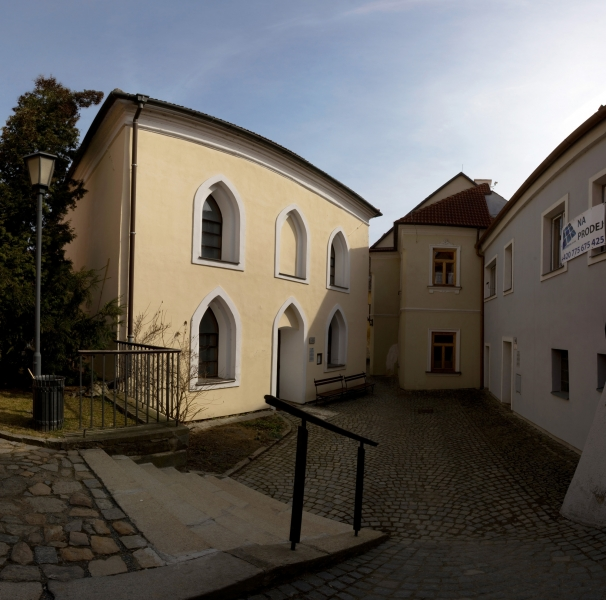
\includegraphics[height=10cm]{../img/predniSynagogaBudova}
	\caption[Přední synagoga \text{[online]} MKS Třebíč. Dostupné z: \url{https://www.mkstrebic.cz/data_5/fotogalerie/15normal.jpg} \text{[cit. 2020-03-26]}]{
		Budova Přední synagogy
	}
	\label{fig:psb}
\end{figure}

\begin{figure}
	\centering
	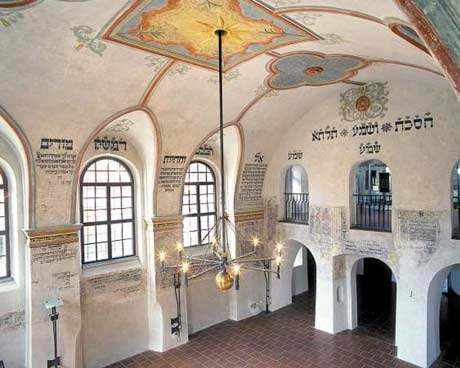
\includegraphics[height=10cm]{../img/zadniSynagogaInterier}
	\caption[Zadní synagoga \text{[online]} Czech tourism. Dostupné z: \url{https://www.czechtourism.com/c/trebic-rear-synagogue/} \text{[cit. 2020-03-27]}]{
		Interiér Zadní synagogy
	}
	\label{fig:zsi}
\end{figure}

\begin{figure}
	\centering
	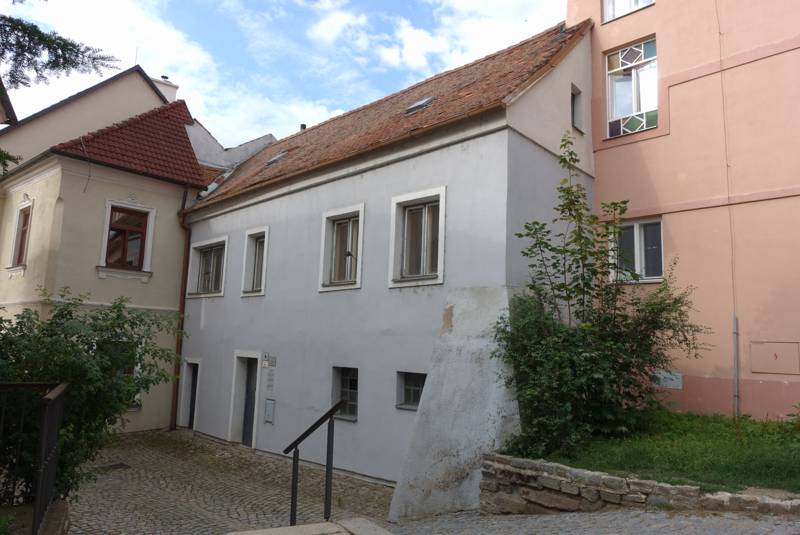
\includegraphics[height=10cm]{../img/rabinuvDumBudova.jpg}
	\caption[Rabínův dům \text{[online]} NPÚ památkový katalog. Dostupné z: \url{https://www.pamatkovykatalog.cz/rabinsky-dum-22238373} \text{[cit. 2020-03-28]}]{
		Rabínův dům
	}
	\label{fig:rdb}
\end{figure}

\begin{figure}
	\centering
	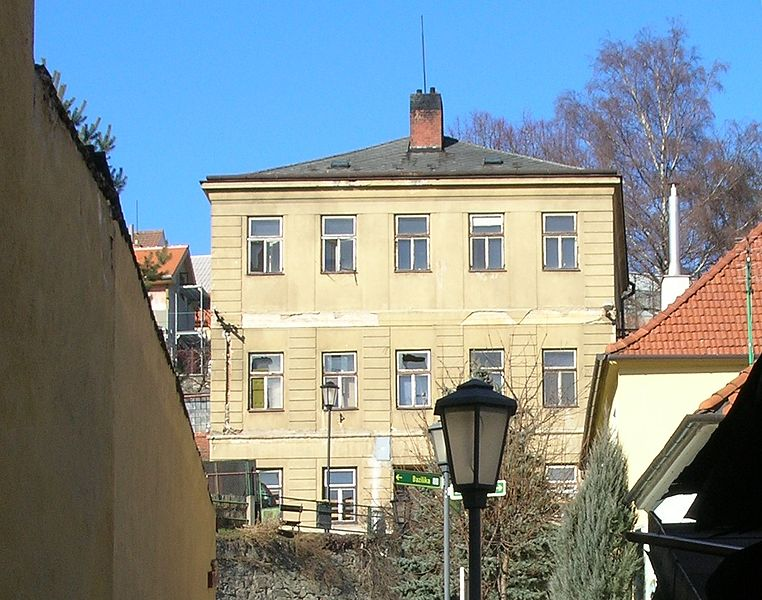
\includegraphics[height=10cm]{../img/zidovskaNemocniceBudova.jpg}
	\caption[Židovská nemocnice \text{[online]} Wikipedia. Dostupné z: \url{https://cs.wikipedia.org/wiki/Soubor:Trebic_zamosti_krankenhaus.jpg} \text{[cit. 2020-03-28]}]{
		Židovská nemocnice
	}
	\label{fig:znb}
\end{figure}

\begin{figure}
	\centering
	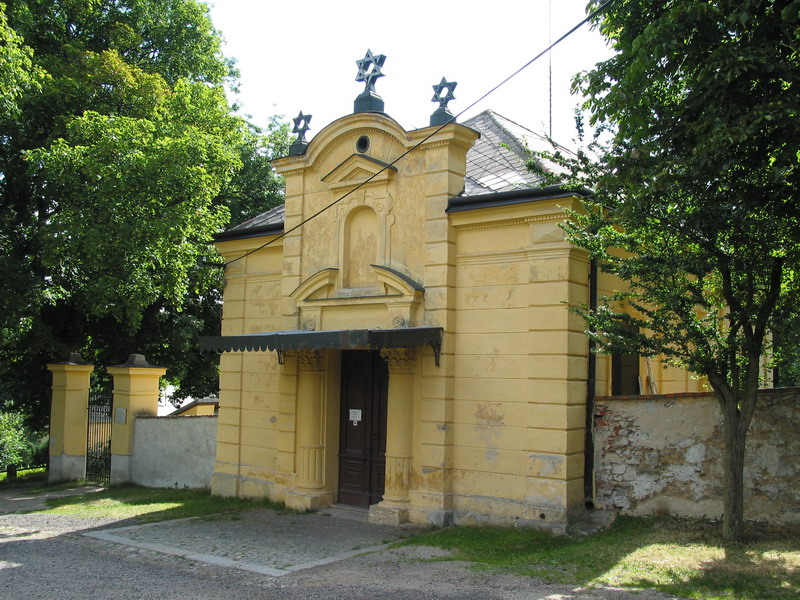
\includegraphics[height=10cm]{../img/zidovskyHrbitov.jpg}
	\caption[Židovský hřbitov \text{[online]} Město Třebíč. Dostupné z: \url{http://www.mesto-trebic.cz/zidovsky-hrbitov.php} \text{[cit. 2020-03-28]}]{
		Židovský hřbitov
	}
	\label{fig:zhh}
\end{figure}

\begin{figure}
	\centering
	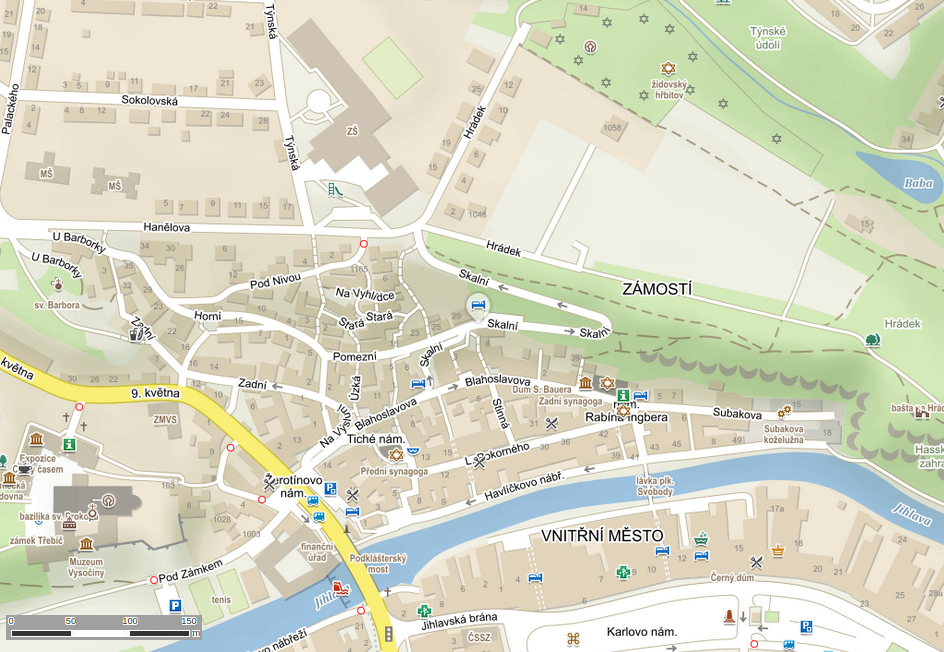
\includegraphics[height=10.5cm]{../img/mapaZidovskehoMesta.png}
	\caption[Mapa Židovského města \text{[online]} Mapy.cz. Dostupné z: \url{https://en.mapy.cz/zakladni?x=15.8789945&y=49.2182114&z=17&source=muni&id=5517} \text{[cit. 2020-03-28], zeditováno}]{
		Mapa Židovského města
	}
	\label{fig:map}
\end{figure}

\chapter*{}

\pagenumbering{roman}
\setcounter{page}{7}

\chapter*{Závěr}
\addcontentsline{toc}{chapter}{Závěr}

Cíl práce se i přes problémy podařilo splnit.
Bohužel se mi díky epidemii CoVid--19 nepodařilo město navštívit a získat tak mé osobní fotografie.
Ty však tvoří jen malou část práce.
Během nočního přejezdu jsem ve městě zastavil a čtvrť alespoň prošel.

Jediný problém ke zpracování představovalo období dějin města od revolučního roku 1848 po současnost.
Bohužel v tomto časovém rozsahu nejsou ani publikace ohledně samotného Třebíče.
Byla sice plánována kniha Třebíč: Dějiny města III., k jejímu vytvoření snad nikdy nedošlo, či vzniklo jen pár výtisků.
Obecně nedostatek středoškolskému studentu přístupných pramenů komplikuje popsat dějiny židovské komunity v Třebíči podrobně.

I tak si myslím, že je výsledkem této práce obstojný souhrnný pohled na historii židovské obce ve Třebíči.
Sám jsem díky této práci získal hluboký náhled do dějin nejen samotného Židovského města, ale i celého Třebíče a Moravy.
Pevně doufám, že se tohoto tématu ujme schopný historik a celé dějiny zmapuje podrobně od začátku do konce.


%%% Seznam použité literatury (bibliografie)
%%%
%%% Pro vytváření bibliografie používáme bibTeX. Ten zpracovává
%%% citace v textu (např. makro \cite{...}) a vyhledává k nim literaturu
%%% v souboru literatura.bib.
%%%
%%% Příkaz \bibliographystyle určuje, jakým stylem budou citovány odkazy
%%% v textu. V závorce je název zvoleného souboru .bst. Styly plainnat
%%% a unsrt jsou standardní součástí latexových distribucí. Styl czplainnat
%%% je dodáván s touto šablonou a bibTeX ho hledá v aktuálním adresáři.

\bibliographystyle{czechiso}    %% Autor (rok) s českými spojkami
% \bibliographystyle{plainnat}    %% Autor (rok) s anglickými spojkami
%\bibliographystyle{unsrt}       %% [číslo]

\renewcommand{\bibname}{Seznam použité literatury}

%%% Vytvoření seznamu literatury. Pozor, pokud jste necitovali ani jednu
%%% položku, seznam se automaticky vynechá.

\bibliography{literatura}

%%% Kdybyste chtěli bibliografii vytvářet ručně (bez bibTeXu), lze to udělat
%%% následovně. V takovém případě se řiďte normou ISO 690 a zvyklostmi v oboru.

% \begin{thebibliography}{99}
%
% \bibitem{lamport94}
%   {\sc Lamport,} Leslie.
%   \emph{\LaTeX: A Document Preparation System}.
%   2. vydání.
%   Massachusetts: Addison Wesley, 1994.
%   ISBN 0-201-52983-1.
%
% \end{thebibliography}


\chapter*{Online zdroje}
\addcontentsline{toc}{chapter}{Online zroje}
\noindent
Historie města Třebíč v datech [online] (2006). stránka města Třebíč. Dostupné z: \url{https://www.trebic.cz/historie\%2Dmesta\%2Dv\%2Ddatech/d-1385/p1=30143} \linebreak[4] [cit. 2020-03-08].

\vspace{0.5cm}
\noindent
POSOLDA, Lukáš. Třebíč na seznamu UNESCO [online] (2003). ARCHiNET. Dostupné z: \url{https://web.archive.org/web/20080307141031/http://www.archinet.cz/index.php?mode=article&art=12912&sec=10019&lang=cz}  [cit. 2020-03-08].

\vspace{0.5cm}
\noindent
BLAŽEK, Poslední žijící třebíčskou Židovku válka ani komunistický režim nešetřily [online] (2020). iDnes. Dostupné z: \url{https://www.idnes.cz/jihlava/zpravy/A200127_529096_jihlava-zpravy_mv} [cit. 2020-03-27].
\listoffigures
\openright
\end{document}
